\documentclass[a4paper,11pt,twoside]{article}
\usepackage[utf8]{inputenc}
\usepackage[left=2.5cm,right=2.5cm, top=3cm, bottom=3cm]{geometry}
\usepackage[dvipsnames]{xcolor}
%\usepackage{xcolor,colortbl}
%\documentclass[xcolor=dvipsnames]{beamer} 
\usepackage{graphicx}
\usepackage{multirow}
\usepackage{enumitem}
%\usepackage[demo]{graphicx}
\usepackage{caption}
\usepackage{subcaption}
%\usepackage{subfig}
\usepackage{graphicx, caption, subcaption}
\usepackage{float}
\usepackage{amsmath}
%\usepackage[english]{babel}
%\usepackage{blindtext}
\usepackage{titlesec}

% for braket notation
\usepackage{mathtools}
\DeclarePairedDelimiter\bra{\langle}{\rvert}
\DeclarePairedDelimiter\ket{\lvert}{\rangle}
\DeclarePairedDelimiterX\braket[2]{\langle}{\rangle}{#1\,\delimsize\vert\,\mathopen{}#2}

%bibliographie
\usepackage{hyperref}
\usepackage{xcolor}

%\usepackage{biblatex}
%\addbibresource{main.bib}
%inhaltsverzeichnis
\setcounter{tocdepth}{2}
\titleformat*{\section}{\huge\bfseries}
\titleformat*{\subsection}{\Large\bfseries}
\titleformat*{\subsubsection}{\large\bfseries}

%Kopf und Fusszeile
\usepackage{fancyhdr}
\pagestyle{fancy}
\setlength{\headheight}{14pt} % Fixes the "headheight too small" warning
\renewcommand{\sectionmark}[1]{\markboth{#1}{}} 
\fancyhf{}
\fancyhead[R]{\textit{Illia Yakushevskyi}} % Put your actual name here
\fancyhead[L]{\leftmark}
\fancyfoot[C]{\thepage}
\renewcommand{\headrulewidth}{0.4pt}

\setcounter{tocdepth}{2} % Keep ToC down to subsections

%everything before is preabmle, doc begins here

\begin{document}
\clearpage
\thispagestyle{empty}
\begin{center}
    \includegraphics[width=8cm,height=8cm,keepaspectratio]{UZH.png}
    \label{fig:uzh}
    
   	\vspace{2cm}
	\Huge
	\textbf{Efficient neural network wave functions for interacting fermions}
	
	\vspace{2cm}
	\huge
	Bachelor Thesis in Physics
	
	\vspace{2cm}	
	\Large
	\textbf{Illia Yakushevskyi}
	
	\vspace{3cm}
	\normalsize	
	Supervised by \\
	\Large
    Prof. Dr. Titus Neupert\\ 
	Dr. Attila Szabó\\
	Ph.D. candidate Simon Hille\\
	
	\vspace{2cm}
	\large
	\today
\end{center}
\vspace{\stretch{3}}
\clearpage
\pagenumbering{roman}
\thispagestyle{plain}
\vspace*{\stretch{1}}
\begin{abstract}

In the last few years, neural network wave functions have proven effective in describing many-body quantum systems. In particular, architectures such as FermiNet, PauliNet, and PsiFormer
have been successful in tackling systems of interacting electrons in quantum chemistry. However,
these all rely on representing antisymmetric fermion wave functions as determinants, whose evaluation may be prohibitively expensive for large systems.
A recently proposed alternative approach implements fermionic antisymmetry using a permutation symmetric neural network extended with a predefined antisymmetric function inspired by fractional quantum Hall states. In principle, such a neural network may be computationally more efficient than the standard approach.

\end{abstract}
\vspace{\stretch{3}}
\clearpage
\newpage
\thispagestyle{plain}
\tableofcontents
\newpage
\listoffigures
\listoftables
\thispagestyle{plain}
\newpage
\stepcounter{page}
\pagenumbering{arabic}
\thispagestyle{plain}
\newpage
\section{Introduction}
\label{sec:intro}

In theoretical condensed matter physics, in order to describe the properties of a material, it is usually sufficient to describe the ground state of the many-body system. However, this has always been a hard task to solve, mainly accomplished by various variational methods. It becomes particularly hard to solve quantum many-body systems which include non-trivial, strongly correlated interactions.
Recently, relatively new approaches to model the wavefunction have emerged, such as Neural Quantum States (NQS)\cite{carleo_solving_2017}. Using it as the ansatz within Variational Monte Carlo (VMC) techniques, together with a finite basis set, has significantly improved the accuracy of the method.



While the computational cost of a bosonic ansatz can scale favorably, encoding the required spin statistics for fermions introduces a major structural challenge. For bosons, one can achieve permutation invariance through simple symmetric pooling, but fermions require a totally antisymmetric wavefunction to satisfy the Pauli Exclusion Principle. This necessitates the use of the Slater determinant, which, using LU decomposition, can be calculated in $O(n^3)$, and can become a bottleneck when training systems with a large number of fermions.

Different methods have been proposed over the years to approach this, such as calculating the Slater determinant or the Pfaffian, or backflow transformations, initially proposed by R. Feynman \cite{feynman_energy_nodate}, and later realised as neural backflow \cite{pfau_ab_2020}.

The Universal Approximation Theorem tells us that with a sufficiently large linear layer and a non-linear activation function we can approximate a function of arbitrary complexity, which sets the premise of this thesis. While Variational Monte Carlo pipeline with NQS training have been implemeted before with Slater determinant, we seek for more efficient representation in terms of computational costs. Certain antisymmetric functions have been only theoreticized before, and this thesis sets to implement one of those antisymmetric representations and rigorously test it's efficiency and general usefulness in practice. 


% epxlain motivation for making separation of parts 

\newpage

% \setcounter{section}{1}



\thispagestyle{plain}


\section{Theoretical Background}

\subsection{Quantum Many-Body Problem in First Quantisation}



Fermions are identical particles whose total wavefunction is antisymmetric under the exchange of any two particles. For two fermions, exchanging particles 1 and 2 must flip the sign of the wavefunction,
\begin{equation}
    \Psi(r_1, r_2) = -\Psi(r_2, r_1).
\end{equation}
Given two single-particle states $\phi_a, \phi_b$, an explicit antisymmetric combination is
\begin{equation}
    \Psi(r_1,r_2) = \frac{1}{\sqrt{2}}\left[\phi_a(r_1)\phi_b(r_2) - \phi_a(r_2)\phi_b(r_1)\right].
\end{equation}
For $N$ fermions this generalizes to the Slater determinant,
\begin{equation}
    \Psi(r_1,...,r_N) = \frac{1}{\sqrt{N!}} \det \begin{pmatrix} \phi_1(r_1) & \cdots & \phi_1(r_N) \\ \vdots & & \vdots \\ \phi_N(r_1) & \cdots & \phi_N(r_N)\end{pmatrix},
\end{equation}
which is antisymmetric, since swapping any two particles swaps two columns of the determinant \cite{griffiths_introduction_2008}.

\cite{orus_practical_2014} For a discrete system of, e.g., $N$ spins-1/2, the dimension of the Hilbert space is $2^N$, which
is exponentially large in the number of particles. Therefore, representing a quantum state of the
many-body system just by giving the coefficients of the wave function in some local basis is an
inefficient representation. The Hilbert space of a quantum many-body system is a really big place
with an incredibly large number of quantum states. Not all quantum states in the Hilbert space of a many-body system are equal: some are more relevant than others.
In particular, one can prove that low-energy eigenstates of gapped Hamiltonians with local interactions obey the so-called area-law for the entanglement entropy. This means that the entanglement entropy of a region of space tends to scale, for large enough regions, as the size of the boundary of the region and not as the volume. And this is a remarkable property, because a quantum state picked at random from a many-body Hilbert space will most likely have an entanglement entropy between subregions that will scale like the volume, and not like the area. In other words, low-energy states of realistic Hamiltonians are not just “any” state in the Hilbert space: they are heavily constrained by locality so that they must obey the entanglement area-law.

\begin{figure}[H]
    \centering
    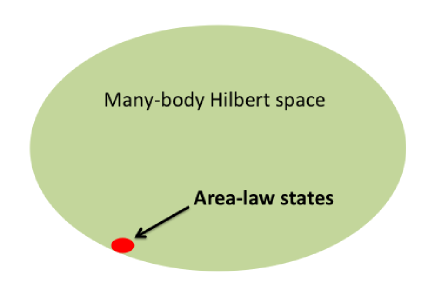
\includegraphics[width=0.5\linewidth]{hilbert_space_corner.png}
    \caption{The physically relevant corner of Hilbert space, reproduced from \cite{orus_practical_2014}.}
    \label{fig:hilbert_corner}
\end{figure}

A broader survey of neural-network wavefunction architectures across this landscape is given in \cite{lange_architectures_2024}.

Literature on the topic has well documented the Fermionic Sign Problem, which appears in VMC setups as a consequence of the Pauli principle and constitutes a big computational challenge for VMC setups. However, in our case this is not a direct concern: we sample directly from $|\psi(x)|^2$ using an explicit variational ansatz, so the sign of $\psi$ is built into the ansatz itself, rather than inferred by the sampler against a bosonic reference. Hence we completely focus on the cost scaling of the antisymmetric part, not on sampling noise from sign cancellation.

Moreover, in our case we work with continuous space, meaning that arguments to our wavefunction are directly the coordinates of the particles, in first quantization, rather than occupation numbers on a fixed lattice or discrete basis set: there is no basis-set truncation error to worry about, the network parametrizes the wavefunction directly, which is exactly the Universal Approximation Theorem argument from the Introduction. It also means sampling must proceed via continuous-space Metropolis moves (Section~\ref{impl:sys}), rather than the discrete-occupation updates used in most lattice NQS work, and that the natural symmetries to exploit are continuous ones (e.g.\ rotations), not discrete lattice symmetries, a point we return to in Section~\ref{sec:results}.
\newpage

\subsection{Variational Monte Carlo}

Since we work in continuous, high dimensional, infite space we can not perform integration to evaluate our wavefunctions. 
Main approach and framework which allows us to postulate wavefunction  $\Psi$, estimate it's local energies, their variance etc by statistical and computational methods is Variational Monte Carlo (VMC).

The base of VMC is the quantum-mechanical variational principle, one of the big advantages of which is that the energy of the system is bounded from below by the ground state energy. By optimizing \ref{sec:SR} our variational state with respect to parameters $\theta$ in order to decrease the energy, we hope to capture an approximation of the ground state, hence capture the correct ground-state behavior.


The known limitation of the method is it's bias to Ansatz, the first assumption of the wavefunction we start optimisation with.
Hence over last 10 years Neural Network Ansatz \ref{sec:nn_ansatz} became increasingly more popular as it is almost always more efficient then starting from the random state.  

Assuming states are orthogonal and normalised, any quantum state $|\psi\rangle$ can be expanded in a basis $\{|x\rangle\}$ as
\begin{equation}
    |\psi\rangle = \sum_x \langle x|\psi\rangle |x\rangle = \sum_x \psi(x)|x\rangle.
\end{equation}
The expectation value of an operator $\hat O$ over this variational state then takes the form
\begin{equation}
    \langle \hat O \rangle = \frac{\langle\psi|\hat O|\psi\rangle}{\langle\psi|\psi\rangle}
    = \frac{\sum_x |\psi(x)|^2 \, O_L(x)}{\sum_x |\psi(x)|^2},
\end{equation}
where we have defined the local estimator of the operator $\hat O$,
\begin{equation}
    O_L(x) = \frac{\langle x|\hat O|\psi\rangle}{\psi(x)}.
\end{equation}
The key point is that $P(x) = |\psi(x)|^2 / \sum_x |\psi(x)|^2$ is a normalised probability distribution. Therefore, the problem of computing the quantum average of $\hat O$ can be rephrased as computing the average of the random variable $O_L(x)$ over samples drawn from $P(x)$:
\begin{equation}
    \langle \hat O \rangle \approx \frac{1}{N}\sum_{n=1}^N O_L(x_n).
\end{equation}

\subsubsection{Stochastic Reconfiguration Driver (SR)}
\label{sec:SR}

A big part of the VMC setup is the VMC driver. We use NetKet's implementation of the \texttt{VMC\_SR} driver and this section will explain it.

Generally, the driver defines a training loop which generates samples with Monte Carlo, evaluates the local energies $E_{loc}$, calculates the gradients, and updates the parameters $\theta$.

The driver we use is called the Stochastic Reconfiguration Driver, with the SR preconditioner \cite{rende_simple_2024, becca_quantum_2017}. The role of SR is to precondition the gradient used in stochastic optimization, improving the convergence rate to the ground state of a Hamiltonian by multiplying the gradients with the inverse of the S matrix.

The S matrix is actually the Quantum Geometric Tensor (QGT). While standard ML optimizers like Adam work in Euclidean parameter space and use the Euclidean norm, the QGT is equipped with a quantum-mechanical distance function, the Fubini-Study distance.
To construct the SR update we will first need the gradient with respect to the variational parameters $\theta$.

We are concerned with the problem of calculating the optimal update to $\theta$, and thus need to solve

\begin{equation}
    \delta \theta = S^{-1} g
\end{equation}

Since the S matrix is symmetric and positive semi-definite, we use Cholesky decomposition to solve for the inverse of the system. In practice, Monte Carlo estimates of $S$ are noisy and can become near-singular, particularly early in training or close to convergence, where the sampled gradients become nearly linearly dependent. To keep the inversion well behaved we add a small multiple of the identity before inverting,
\begin{equation}
    S \rightarrow S + \lambda I,
\end{equation}
a parameter we call the diagonal shift $\lambda$: it trades a small bias in the update direction for a much better-conditioned inverse. The concrete values used and how they were tuned are given in Section~\ref{impl:sys}.

Together, the variational principle, the local-energy estimator, and the SR-preconditioned update give us the full VMC machinery: sample from $|\psi_\theta(x)|^2$, estimate $E_{loc}(x)$ and its gradient, and take a natural-gradient step towards lower energy. What remains is the choice of $\psi_\theta$ itself (the neural network ansatz), which is the subject of the rest of this chapter.

\newpage


\subsection{Neural Network Ansatz for Fermions}
\label{sec:nn_ansatz}

For fermions, efficiently representing antisymmetric states remains a major challenge. The standard approach is to expand $\Psi$ in terms of Slater determinants constructed from a single-particle basis set $\phi_1(r), ..., \phi_L(r)$.
The problem with the Slater determinant is that it scales exponentially with the number of particles $N$. From the perspective of computational cost, it translates to $O(n^3)$ complexity, when solving the Slater determinant with LU decomposition. The main goal of this thesis is to verify an ansatz alternative to the Slater determinant, which could bring down the computational cost to $O(n^2)$, thus being a more efficient representation for fermionic wavefunctions. Such an ansatz was first proposed to use a symmetrical part and an antisymmetric part as arguments to a neural network \cite{fu_minimal_2025}.

\begin{equation}
\psi(r_1 ,..., r_n) = \Psi( r_1, ...,r_n,  \eta(r_1 ,..., r_n  ))
\end{equation}


Where $\Psi$ is implemented as a Neural Network. While we know how to make a symmetrized Ansatz for the bosonic case (Section~\ref{tab:deepsets}), the challenge is to construct the so-called \textit{signature encoder}:

\begin{equation}
    \eta = \prod_{1 \le j < i \le N} (x_i - x_j)
\end{equation}

This is the Vandermonde determinant of the coordinates $x_1,...,x_N$ (equivalently, $\det[x_i^{k-1}]_{i,k=1}^N$): antisymmetric by construction, and vanishing exactly when two coordinates coincide.

This particular choice is not arbitrary. Any totally antisymmetric function $F(x_1,...,x_N)$ can be written as
\begin{equation}
    F(x_1,...,x_N) = \eta(x_1,...,x_N) \cdot g(x_1,...,x_N)
\end{equation}
for some symmetric function $g$: both $F$ and $\eta$ flip sign under every transposition of two particles, so their ratio $F/\eta$ is invariant under every transposition, wherever $\eta \neq 0$, and hence symmetric under the full permutation group. 
In this sense, the construction $\psi = \Psi(\xi, \eta)$ is universal: for a sufficiently expressive $g$ (played here by the network $\Psi$), it can in principle represent \emph{any} fermionic wavefunction, including the Slater determinant itself. This is exactly the claim in \cite{fu_minimal_2025}, and the general strategy of dressing a Vandermonde-type factor with a symmetric function is also what underlies the Laughlin wavefunctions of the fractional quantum Hall effect mentioned in the Abstract.

Whether that representational universality is actually reachable by gradient-based training from a random initialization is a separate question. We show in Section~\ref{sec:lazy_trap} that it is not, in general: the $g$ needed to reproduce a generic Slater determinant from $\eta$ is not smooth at particle collisions, unlike the trivial choice $g \equiv \text{const}$, which is why the network finds the latter and gets stuck there.

This can be extended to two dimensions using complex coordinates.

\begin{equation}
    \eta = \eta_1 + i \eta_2 = \prod_{1 \le j < i \le N} (z_i - z_j)
\end{equation}


Later in this work we use a regularised version of $\eta$ for stability at the nodes, i.e. when $|z_i - z_j| \rightarrow 0$:

\begin{equation}
\label{eq:eta}
\eta = \prod_{1 \le j < i \le N} \frac{z_i - z_j}{\sqrt{|z_i - z_j|^2 + a^2}}
\end{equation}

\subsubsection{Deep Sets}
\label{tab:deepsets}

For bosons, the wavefunction must be symmetric, rather than antisymmetric, under particle exchange. The natural architecture for this is Deep Sets \cite{zaheer_deep_2018}: each particle is passed through a shared per-particle encoder $\phi$, the resulting per-particle features are pooled (summed) into a single vector, and a decoder $\rho$ maps that pooled vector to the output,
\begin{equation}
    f(r_1, ..., r_N) = \rho\left(\sum_{i=1}^N \phi(r_i)\right).
\end{equation}
Since summation does not depend on the order of its terms, $f$ is automatically symmetric under any permutation of the particles, regardless of what $\phi$ and $\rho$ are. This is exactly the symmetric part $\xi$ used in the FermiSets construction above: $\xi(r_1,...,r_N) = \sum_i \phi(r_i)$, evaluated by the same shared encoder for both the $+\eta$ and $-\eta$ branches.

\subsubsection{Slater-Determinant Baseline (SlaterNN)}
\label{sec:slaternn}

As a direct baseline for comparison, we also implement a standard Slater-determinant ansatz with neural-network orbitals, without any backflow: a single shared per-particle MLP produces $N$ orbitals $\phi_k(r_i)$ per particle, and the wavefunction is the determinant of the resulting $N \times N$ matrix,
\begin{equation}
    \psi(r_1,...,r_N) = \det\left[\phi_k(r_i)\right]_{i,k=1}^N,
\end{equation}
evaluated via \texttt{slogdet} for numerical stability. This is the $O(n^3)$ reference our FermiSets construction is compared against throughout Section~\ref{sec:results}: same envelope convention, same training pipeline; only the antisymmetrization mechanism differs.

\subsubsection{The Lazy-State Trap}
\label{sec:lazy_trap}

We will discuss this further in the Results section (\ref{sec:results}), but the following must be mentioned now. The construction above has a shortcut built into it. For any smooth symmetric function $g(\xi)$, the state

\begin{equation}
    \psi(r_1,...,r_N) = \eta(r_1,...,r_N) \cdot g(\xi(r_1,...,r_N)) \cdot e^{-\sum_i r_i^2/2}
\end{equation}

is automatically antisymmetric, since $\eta$ already flips sign under every particle exchange. The network does not have to learn anything about the sign structure to satisfy the Pauli principle: it can simply ignore the phase of $\eta$ and output a plain symmetric prefactor. This creates a bias towards the lazy-state trap, a property of the ansatz itself that will cause trouble in the actual implementation, discussed further below.

The simplest such choice, $g \equiv \text{const}$, turns out to be an exact eigenstate of the non-interacting Hamiltonian. Writing particle positions as complex numbers $z_i = x_i + i y_i$, the signature encoder for $\dim=2$ is the complex Vandermonde determinant

\begin{equation}
    \eta = \prod_{i<j} (z_i - z_j) = \det \begin{pmatrix} 1 & 1 & \cdots & 1 \\ z_1 & z_2 & \cdots & z_N \\ \vdots & & & \vdots \\ z_1^{N-1} & z_2^{N-1} & \cdots & z_N^{N-1} \end{pmatrix},
\end{equation}

which is exactly the Slater determinant built from the single-particle orbitals $1, z, z^2, ..., z^{N-1}$.

It is worth being explicit about the word \textit{holomorphic}, since it carries the whole argument. Packing the two real coordinates into $z_i = x_i + i y_i$ throws nothing away: together with its conjugate $\bar z_i = x_i - i y_i$ it recovers the originals through $x_i = (z_i + \bar z_i)/2$ and $y_i = (z_i - \bar z_i)/2i$, so any function of the pair $(x_i, y_i)$ is equally a function of the pair $(z_i, \bar z_i)$. A function is called \textit{holomorphic} when, written this way, it depends on $z$ alone and not at all on $\bar z$ (equivalently $\partial f / \partial \bar z = 0$, the Cauchy-Riemann condition); this is exactly the class of complex-differentiable functions, namely the powers $z, z^2, z^3, \dots$ and any polynomial or power series in $z$. Its mirror image, an \textit{antiholomorphic} function, depends on $\bar z$ alone and is precisely the complex conjugate of a holomorphic one. The distinction is physical, not just bookkeeping: in polar coordinates $z^k = r^k e^{ik\theta}$, so a holomorphic orbital carries a definite, positive angular momentum $L_z = +k\hbar$, whereas its antiholomorphic partner $\bar z^k = r^k e^{-ik\theta}$ carries the opposite, $L_z = -k\hbar$. The Vandermonde determinant is assembled entirely from holomorphic orbitals, and it is this one-sided, maximally-rotating character that makes it both effortless for the network to reach and, as we return to in Section~\ref{sec:results}, exactly degenerate with a mirror-image state of opposite total angular momentum.

Each orbital $z^k$ is thus an eigenstate of the 2D harmonic oscillator with energy $\hbar\omega(k+1)$, carrying all $k$ of its quanta as angular momentum ($n = n_x + n_y = k$). Filling the lowest $N$ of them (aufbau) gives the total energy of this state as

\begin{equation}
    E_{\text{lazy}} = \hbar\omega \sum_{k=0}^{N-1} (k+1) = \hbar\omega\, \frac{N(N+1)}{2}.
\end{equation}

Because $E_\text{lazy}$ is a true eigenvalue of $\hat H$, this state is an exact stationary point of the energy expectation value $\langle \psi | \hat H | \psi\rangle / \langle \psi|\psi\rangle$ \cite{becca_quantum_2017}: the energy gradient vanishes there identically, for any architecture, no matter what it is in principle capable of representing elsewhere. Gradient-based VMC has no local incentive to leave this state once it lands there. And since $g \equiv \text{const}$ is the easiest possible function to reach from a random initialization, it lands there almost every time. We call this the \textit{lazy-state trap}: not a failure of expressivity, but of trainability: the network can represent the true ground state (we show this directly in Section~\ref{sec:results}), it just has no gradient telling it to go there.

Nothing in this argument is specific to the isotropic harmonic trap. The trapped family, more generally, consists of any state whose antisymmetric part is a product of pairwise coordinate differences, what we call a \textit{sortable} sign structure, since it is exactly the sign structure a sorting of the particles would produce. The true 2D ground state instead has a sign structure built from a signed area (e.g.\ $\det\{1,x,y\}$ for $N=3$), which cannot be factored into pairwise terms. It is this genuinely two-dimensional antisymmetry, not the harmonic potential specifically, that the ansatz fails to reach unaided: we confirm this by repeating the experiment on a potential with no rotational symmetry to lean on, in Section~\ref{sec:results}. That section also presents two structural ways to escape the trap without ever knowing the true ground state in advance.

\newpage



\section{Implementation and Experimental Setup}

In this section we going to state the particular system we test the Ansatz with, and all the computational parameters involved. 

First of all, we need a localized Hamiltonian, and it's very convenient to use the Quantum Harmonic Oscillator as the simplest and theoretically solvable system. Then we need to initiate a continuous Hilbert space in two dimensions (the main focus of our thesis) and then spawn the chains which will sample the coordinates for our Hamiltonian. Since the Hilbert space is vast, we must be smart about how we draw the coordinates for it, so we use the Metropolis algorithm to only sample the most relevant points, where the wavefunction is most probable to reside. Then we need to feed the sampled coordinates to the neural network Ansatz and estimate the local energy with VMC. After the weights of the neural network are optimized to minimize the local energy, the loop repeats by proposing new coordinates. 

Within this loop there are several classes in which our code is divided: \texttt{System} ,\texttt{FermiSets},\texttt{Trainer} and they are worth explaining in the following subsections. 

Simulations for this work were performed using
NetKet \cite{carleo_netket_2019, vicentini_netket_2022}. This software is built on top of JAX~\cite{bradbury_jax_2018}
and Flax~\cite{heek_flax_2024}.

The configuration file for the canonical benchmark experiment (\texttt{Experiment}\footnote{\url{https://github.com/IlyaYakushevskiy/FermiNQS/blob/main/configs/experiment/qho_fermisets_2d_3N_bench.yaml}}) and the ansatz implementation (\texttt{Ansatz}\footnote{\url{https://github.com/IlyaYakushevskiy/FermiNQS/blob/main/src/ansatz.py}}) are both available online.




\subsection{System}
\label{impl:sys}

The object \textbf{System} includes a description of the continuous Hilbert space we work with, its dimension, and the Hamiltonian for which we solve Schrödinger's equation. Concretely, this Hilbert space is NetKet's \texttt{Particle} Hilbert space over free space (no periodic boundary conditions are implemented). It's worth noting that antisymmetrization of the state is enforced by the Ansatz (Neural Quantum State), not by the System.

For $N$ particles of mass $m$ in $\texttt{dim}$ dimensions, the Hamiltonian we solve throughout this thesis is
\begin{equation}
\label{eq:hamiltonian}
\hat{H} = \sum_{i=1}^{N} \left[ -\frac{\hbar^{2}}{2m}\nabla_i^{2} \right] + V(r_1,...,r_N),
\end{equation}
a fixed kinetic-energy operator (\texttt{mass} sets $m$, kept at 1 throughout) plus a potential term $V$ that varies between experiments. Three potentials are implemented, selected via \texttt{system.potential}:
\begin{itemize}
    \item \texttt{qho\_no\_inter}: the isotropic harmonic trap, $V(x) = \frac{1}{2}\sum_i r_i^2$, the main benchmark system throughout this thesis. Its appeal is that the exact ground state is known in closed form for any $N$ (Section~\ref{sec:results}), so any discrepancy between our variational energy and the true one is unambiguously the ansatz's fault, not a reference-energy uncertainty. We specifically benchmark at closed-shell particle numbers ($N=3,6,10,\dots$), where the ground state is non-degenerate; open shells (e.g.\ $N=4$) have a degenerate ground state and give a flat direction in the loss that confounds convergence diagnostics, as we show directly in Section~\ref{sec:results}.
    \item \texttt{qho\_aniso}: an anisotropic trap, $V(x) = \frac{1}{2}\sum_i (x_i^2 + \omega_y^2 y_i^2)$, controlled by \texttt{system.omega\_y}. It remains exactly solvable (still separable into independent $x$ and $y$ oscillators) while breaking rotational symmetry outright, which is precisely what makes it useful: it tests whether the ansatz's behaviour on the isotropic trap is a generic property of the architecture, or an artifact of the extra symmetry the isotropic trap happens to have.
    \item \texttt{dot\_gauss}: an interacting quantum dot, the trap plus a Gaussian repulsion $\lambda \sum_{i<j} \exp(-r_{ij}^2/2s^2)$, controlled by \texttt{system.int\_strength} ($\lambda$) and \texttt{system.int\_range} ($s$). We use a Gaussian repulsion rather than the bare Coulomb $1/r_{ij}$ deliberately: it has no coalescence cusp, so a smooth neural network is not handicapped relative to the exact solution from the start, and its two-body matrix elements in the oscillator basis are numerically exact, so the same operator can be used identically in both the VMC ansatz and the exact-diagonalization reference (Section~\ref{sec:diagnostics}) with no discretization mismatch between the two. This system has no closed-form ground state, so the reference energy \texttt{system.e\_ref} must be supplied from that exact diagonalization instead.
\end{itemize}

\texttt{N} and \texttt{dim} in Equation~\ref{eq:hamiltonian} are config keys directly; this thesis focuses on \texttt{dim=2}.





\subsection{Sampler and Trainer}

The Sampler proposes new particle coordinates via a custom Metropolis rule, \texttt{SamplerExchangeRule}, mixing two kinds of moves:
\begin{itemize}
    \item a Gaussian drift, $r \rightarrow r + \sigma \cdot \mathcal{N}(0,1)$, with step size \texttt{sampler.sigma};
    \item a particle-exchange move, swapping the full coordinates of two randomly chosen particles, proposed with probability \texttt{sampler.exchange\_prob}.
\end{itemize}

Since $|\psi(x)|^2$ is exactly permutation-symmetric for any antisymmetric $\psi$, exchange moves are always accepted: they carry no information about the sign of $\psi$. Their role is purely to improve mixing: without them, unwinding two particles that have drifted close to each other would require many small Gaussian steps, so exchange moves let the chains decorrelate much faster.

\texttt{sampler.sigma} is auto-tuned at the start of training (\texttt{sampler.tune\_sigma}) to target an acceptance rate between 30\% and 60\%: acceptance outside this window signals a step size that is too small (slow mixing) or too large (most moves rejected). Mixing quality itself is monitored via two standard MCMC diagnostics that NetKet computes automatically on every reported estimate: $\hat R$, the Gelman-Rubin statistic across chains (close to 1 for well-mixed chains), and the integrated autocorrelation time. \texttt{sampler.n\_chains} sets the number of independent chains run in parallel: more chains reduce the correlation between the samples used in a single gradient estimate, at the cost of GPU memory. \texttt{sampler.sweep\_size} is the number of proposed moves per chain between recorded samples.

The Trainer wraps NetKet's VMC driver and everything needed to run it to convergence:
\begin{itemize}
    \item \texttt{trainer.lr} is the base learning rate, decayed exponentially with rate \texttt{trainer.lr\_decay\_rate} every \texttt{trainer.lr\_decay\_steps} iterations.
    \item \texttt{trainer.optimizer} selects between \texttt{sgd}, \texttt{momentum} (with \texttt{trainer.momentum\_beta}), and plain \texttt{adam}, we compare those optmizers later in apendix \ref{sec:solver}.
    \item \texttt{trainer.vmc\_iters} is the number of training iterations; \texttt{trainer.n\_samples} and \texttt{trainer.n\_discard\_per\_chain} set the number of Monte Carlo samples used per gradient step and the burn-in discarded from the start of each chain.
    \item \texttt{trainer.diag\_shift} is the diagonal shift $\lambda$ introduced in Section~\ref{sec:SR}; \texttt{trainer.pinv\_rtol}/\texttt{pinv\_atol} control the tolerance of the Cholesky-based solver used to invert the (shifted) S matrix.
    \item \texttt{trainer.chunk\_size} splits the batch of samples into smaller chunks for the forward/backward pass, trading speed for GPU memory, necessary since the S matrix scales as (number of samples)$^2$ under the kernel trick (\texttt{use\_ntk=True}) used throughout.
\end{itemize}

Two safety mechanisms sit around the driver:
\begin{itemize}
    \item a trust-region rescaling of the SR step: if the natural-gradient step's squared norm $\langle \delta\theta | S | \delta\theta\rangle$ exceeds a fixed threshold (hardcoded to 900), the step is rescaled down rather than discarded, guarding against ill-conditioned updates without freezing training entirely.
    \item an auto-rollback guard (\texttt{trainer.auto\_rollback}): if the energy becomes non-finite, or exceeds the best value seen so far by more than \texttt{trainer.rollback\_margin} (or $5\sigma$ of the local-energy variance, whichever is larger), training stops, the parameters are restored from the last good checkpoint, the learning rate is halved, and training resumes, up to \texttt{trainer.max\_retries} times.
\end{itemize}

Whenever \texttt{trainer.validation} is enabled, every 50 steps the current parameters are checkpointed to disk and re-evaluated on a freshly seeded, independent Markov chain (decorrelated from the training chain) to get an unbiased ``Validation Energy'' alongside the (potentially autocorrelated) training-chain estimate. This is the number reported throughout Section~\ref{sec:results}.

Two further optional training-time penalties (\texttt{trainer.holo\_penalty}/\texttt{deflation\_penalty} and their associated hyperparameters) exist for one exploratory trap-escape approach discussed as future work in Section~\ref{sec:conclusions_outlook}; they are not used in the ansatz's main results.


\subsection{Neural Network Ansatz}

As introduced in Section~\ref{sec:nn_ansatz}, the FermiSets ansatz is built from a symmetric Deep Sets embedding $\xi$ and the antisymmetric signature encoder $\eta$; Figure~\ref{fig:fermisets_architecture} shows the resulting computational graph. Particle coordinates enter as a batch of shape $(\text{batch}, N, \texttt{dim})$, and for the $\texttt{dim}=2$ systems this thesis focuses on, each particle contributes a pair $(x_i,y_i)$, packed into $z_i = x_i + iy_i$. From these raw coordinates, $\eta(R)$, the regularised complex Vandermonde determinant of Equation~\ref{eq:eta}, is computed directly: it is the only antisymmetric part in the entire network, everything else is built to be exchange-symmetric. In parallel, each particle's coordinates pass through the same shared encoder $\phi$, are summed over particles (the permutation-symmetric pooling step of the Deep Sets construction), and the pooled vector is passed through a decoder $\rho$ to give $\xi(R)$, a fixed size, permutation-invariant summary of the whole configuration regardless of $N$.

$\xi(R)$ is concatenated with $\mathrm{Re}(\eta)$ and $\mathrm{Im}(\eta)$ and fed into a single, generously wide layer, rather than several narrower stacked ones. This is a deliberate choice rather than a default: the Universal Approximation Theorem (Section~\ref{sec:intro}) already guarantees that one sufficiently wide layer with a non-linearity can approximate the function we need, and empirically, adding an extra stacked layer here made training roughly $30\times$ slower per iteration for no accuracy benefit (Appendix~\ref{app:ablations}). Within this VMC setup, shallow and wide outperforms deep in practice, and the theorem gives us license to prefer it.

This wide layer, the $\Psi$-net, is evaluated twice with shared weights, once at $+\eta$ and once at $-\eta$, giving two log-amplitudes $\Psi_0(\xi,\eta)$ and $\Psi_0(\xi,-\eta)$, which are then combined explicitly as
\begin{equation}
    \Psi(\xi,\eta) = \tfrac{1}{2}\big[\Psi_0(\xi,\eta) - \Psi_0(\xi,-\eta)\big],
\end{equation}
computed in log-space via a signed log-sum-exp for numerical stability, though this equation is exactly what it computes. This subtraction is the step that actually enforces the fermionic sign flip: nothing upstream of it is antisymmetric under particle exchange on its own. The network finally returns $\log\psi$, split into a log-modulus and a phase channel, never $\psi$ itself: NetKet's variational-state machinery expects log-amplitudes, and $|\psi|$ can span many orders of magnitude across a batch, so exponentiating anywhere inside the network would overflow long before that.

The relevant parameters:
\begin{itemize}
    \item \texttt{N} is the number of particles in the system.
    \item \texttt{dim} is the dimension of the continuous Hilbert space.
    \item \texttt{hidden\_units} is the width of $\phi$ and $\rho$ (the encoder/decoder hidden layers).
    \item \texttt{out\_units} is the width of the final $\Psi$ head, split evenly between the log-modulus and phase channels.
    \item \texttt{pretrained\_path} loads a previous run's checkpoint to warm-start training, instead of a random initialization.
\end{itemize}

Two accepted config keys, \texttt{pool\_fct\_name} and \texttt{L}, are currently unused in the implementation, reserved for a pooling-function choice that was never needed in practice.

The regularisation constant $a$ in the regularised signature encoder (Equation~\ref{eq:eta}) is currently hardcoded to $1.0$ inside \texttt{eta\_antisymmetric} rather than exposed as a config key.

Note that \texttt{sampler.n\_chains}, \texttt{trainer.n\_samples}, and \texttt{trainer.chunk\_size} do not affect the ansatz's own input size: they control how many samples are evaluated in parallel (the batch dimension), not the feature dimension. The ansatz's actual input, per sample, is the flattened vector of all particle coordinates, of size $N \times \texttt{dim}$.



\begin{figure}[H]
    \centering
    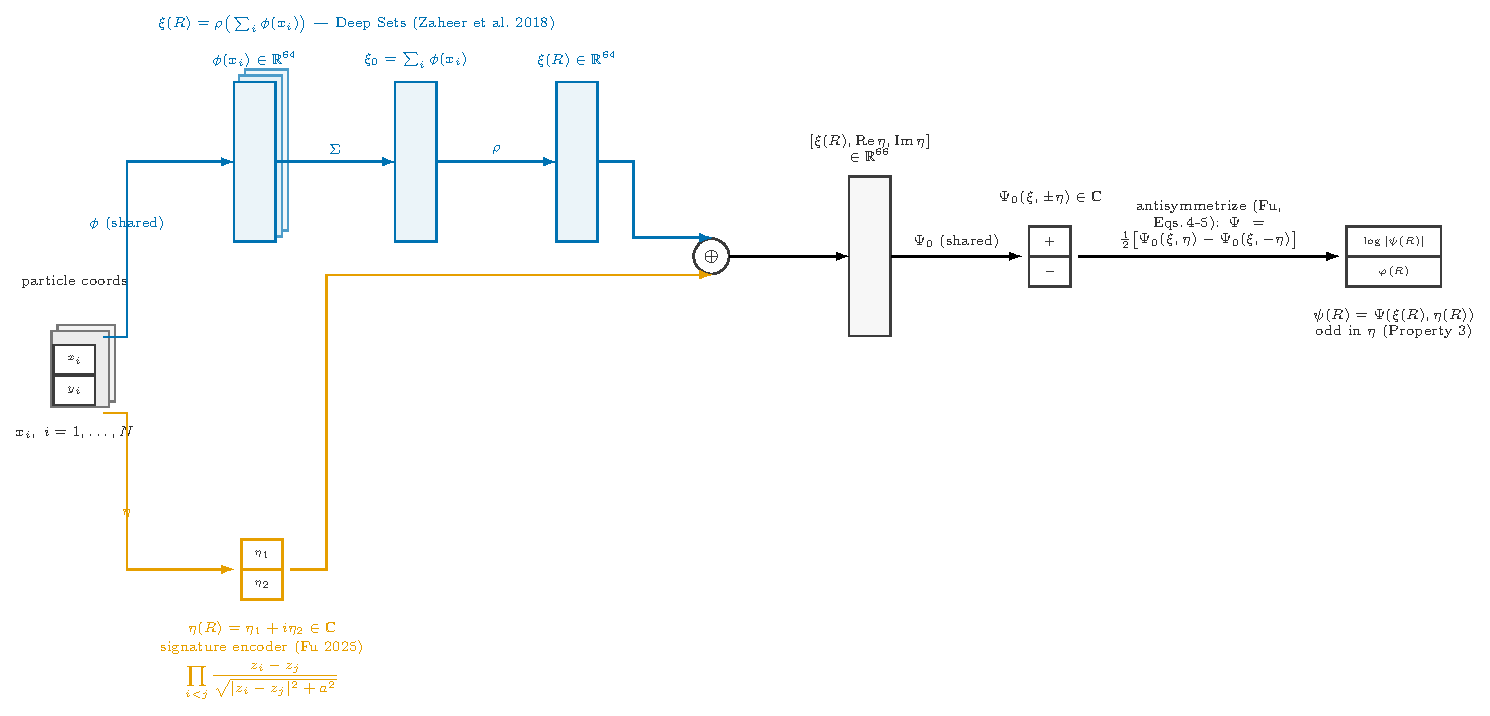
\includegraphics[width=1\linewidth]{fermisets_architecture.pdf}
    \caption{FermiSets architecture: shared per-particle encoder $\phi$, symmetric pooling and decoder $\rho$ producing $\xi$, combined with the signature encoder $\eta$ in the $\Psi$ head.}
    \label{fig:fermisets_architecture}
\end{figure}


\newpage

\section{Results $\&$ Discussion}
\label{sec:results}

In this section we will present results of our numerous experiments. As the first runs showed FermiSets to be unreliable in converging, we will expand here on the ways to isolate the problem, and systematically improve convergence. 
From a random start the FermiSets ansatz converges to one specific wrong state; we identify that state exactly and show it is a structural trap of the architecture, not a tuning artefact; we then present the one structural remedy that removes it, and the point at which a second, unrelated obstacle takes over and the remedy stops helping. All experiments use the systems of Section~\ref{impl:sys}.

Whenever we claim the network has fallen into the trap, we quantify it by the squared overlap (fidelity) of the trained state $\psi$ with an analytic reference state $\phi$,
\begin{equation}
    \mathcal{F}[\psi,\phi] = \frac{|\langle \psi | \phi \rangle|^2}{\langle \psi|\psi\rangle\,\langle \phi|\phi\rangle},
    \label{eq:fidelity}
\end{equation}
estimated by importance sampling from a Gaussian reference distribution.

\subsection{The trap}
\label{sec:n3_trap}

We start from three spinless fermions in the isotropic harmonic trap of Section~\ref{impl:sys}, that is Equation~\ref{eq:hamiltonian}  with $N=3$, \texttt{qho\_no\_inter},  $\hbar = m = \omega = 1$, 

\begin{equation}
\hat{H}_0
=
\sum_{i=1}^{3}
\left[
    -\frac{\hbar^{2}}{2m}\nabla_i^{2}
    + \frac{1}{2} m \omega^{2} \mathbf r_i^{2}
\right].
\end{equation}

In the two-dimensional trap the single-particle shells $n = n_x + n_y$ have degeneracy $n+1$, so three fermions fill the shells $n=0$ and $n=1$ exactly and close them, hence many-body ground state is unique, with energy $E_0 = \hbar\omega\,(1 + 2 + 2) = 5\,\hbar\omega$ and total angular momentum $L_z = 0$


What training actually does is collected in Figure~\ref{fig:n3_trap}. From random initial parameters the energy falls steeply out of its initial value near $7.5\,\hbar\omega$ and settles shortly onto a plateau at $E = 6.0022 \pm 0.0026$ averaged over the last hundred iterations, and it does not leave that plateau again for the remainder of the run. Every diagnostic we have says this run is healthy. The variance of the local energy falls from $4.3$ to $0.024$, which is precisely the signature of an exact eigenstate, whose local energy is constant across configurations. The independently reseeded validation chain agrees with the training estimate inside its error bar, $6.0041 \pm 0.0028$ at iteration $350$, so the plateau is not an autocorrelation artefact of the training sampler; the acceptance rate holds at $0.87$ and $\hat R$ stays between $1.07$ and $1.10$ throughout. The trust-region rescaling of the stochastic-reconfiguration step never engages either, the bilinear form remaining in the range $8$ to $16$ against its threshold of $900$, so the optimiser is not being quietly truncated. By every criterion one would ordinarily apply to a variational run, this run has converged.

It has converged to the first excited state above the ground state with value $6 = N(N+1)/2$ is the exact eigenvalue of the holomorphic Vandermonde state introduced in Section~\ref{sec:lazy_trap}, the state $\det[1, z, z^2]\,e^{-r^2/2}$ whose antisymmetric factor is the complex Vandermonde $\prod_{i<j}(z_i - z_j)$, which is exactly our signature encoder $\eta$ itself. The overlap metrics confirm the identification. Against the analytic ground state the trained wavefunction has $\mathcal{F} = 10^{-6}$, no ground-state content whatsoever, while against the holomorphic state it has $\mathcal{F} = 0.85$. 

This state is also known a in the field as Lowest Landau Level (LLL)  $\nu = 1$ Laughlin wavefunction $\Psi_{LL} = \prod_{i<j}(z_i - z_j)^q\,e^{-\sum|z_i|^2/2}$ at $q=1$, that is the filled lowest Landau level transplanted from a magnetic field into the harmonic trap. 

\begin{figure}[H]
    \centering
    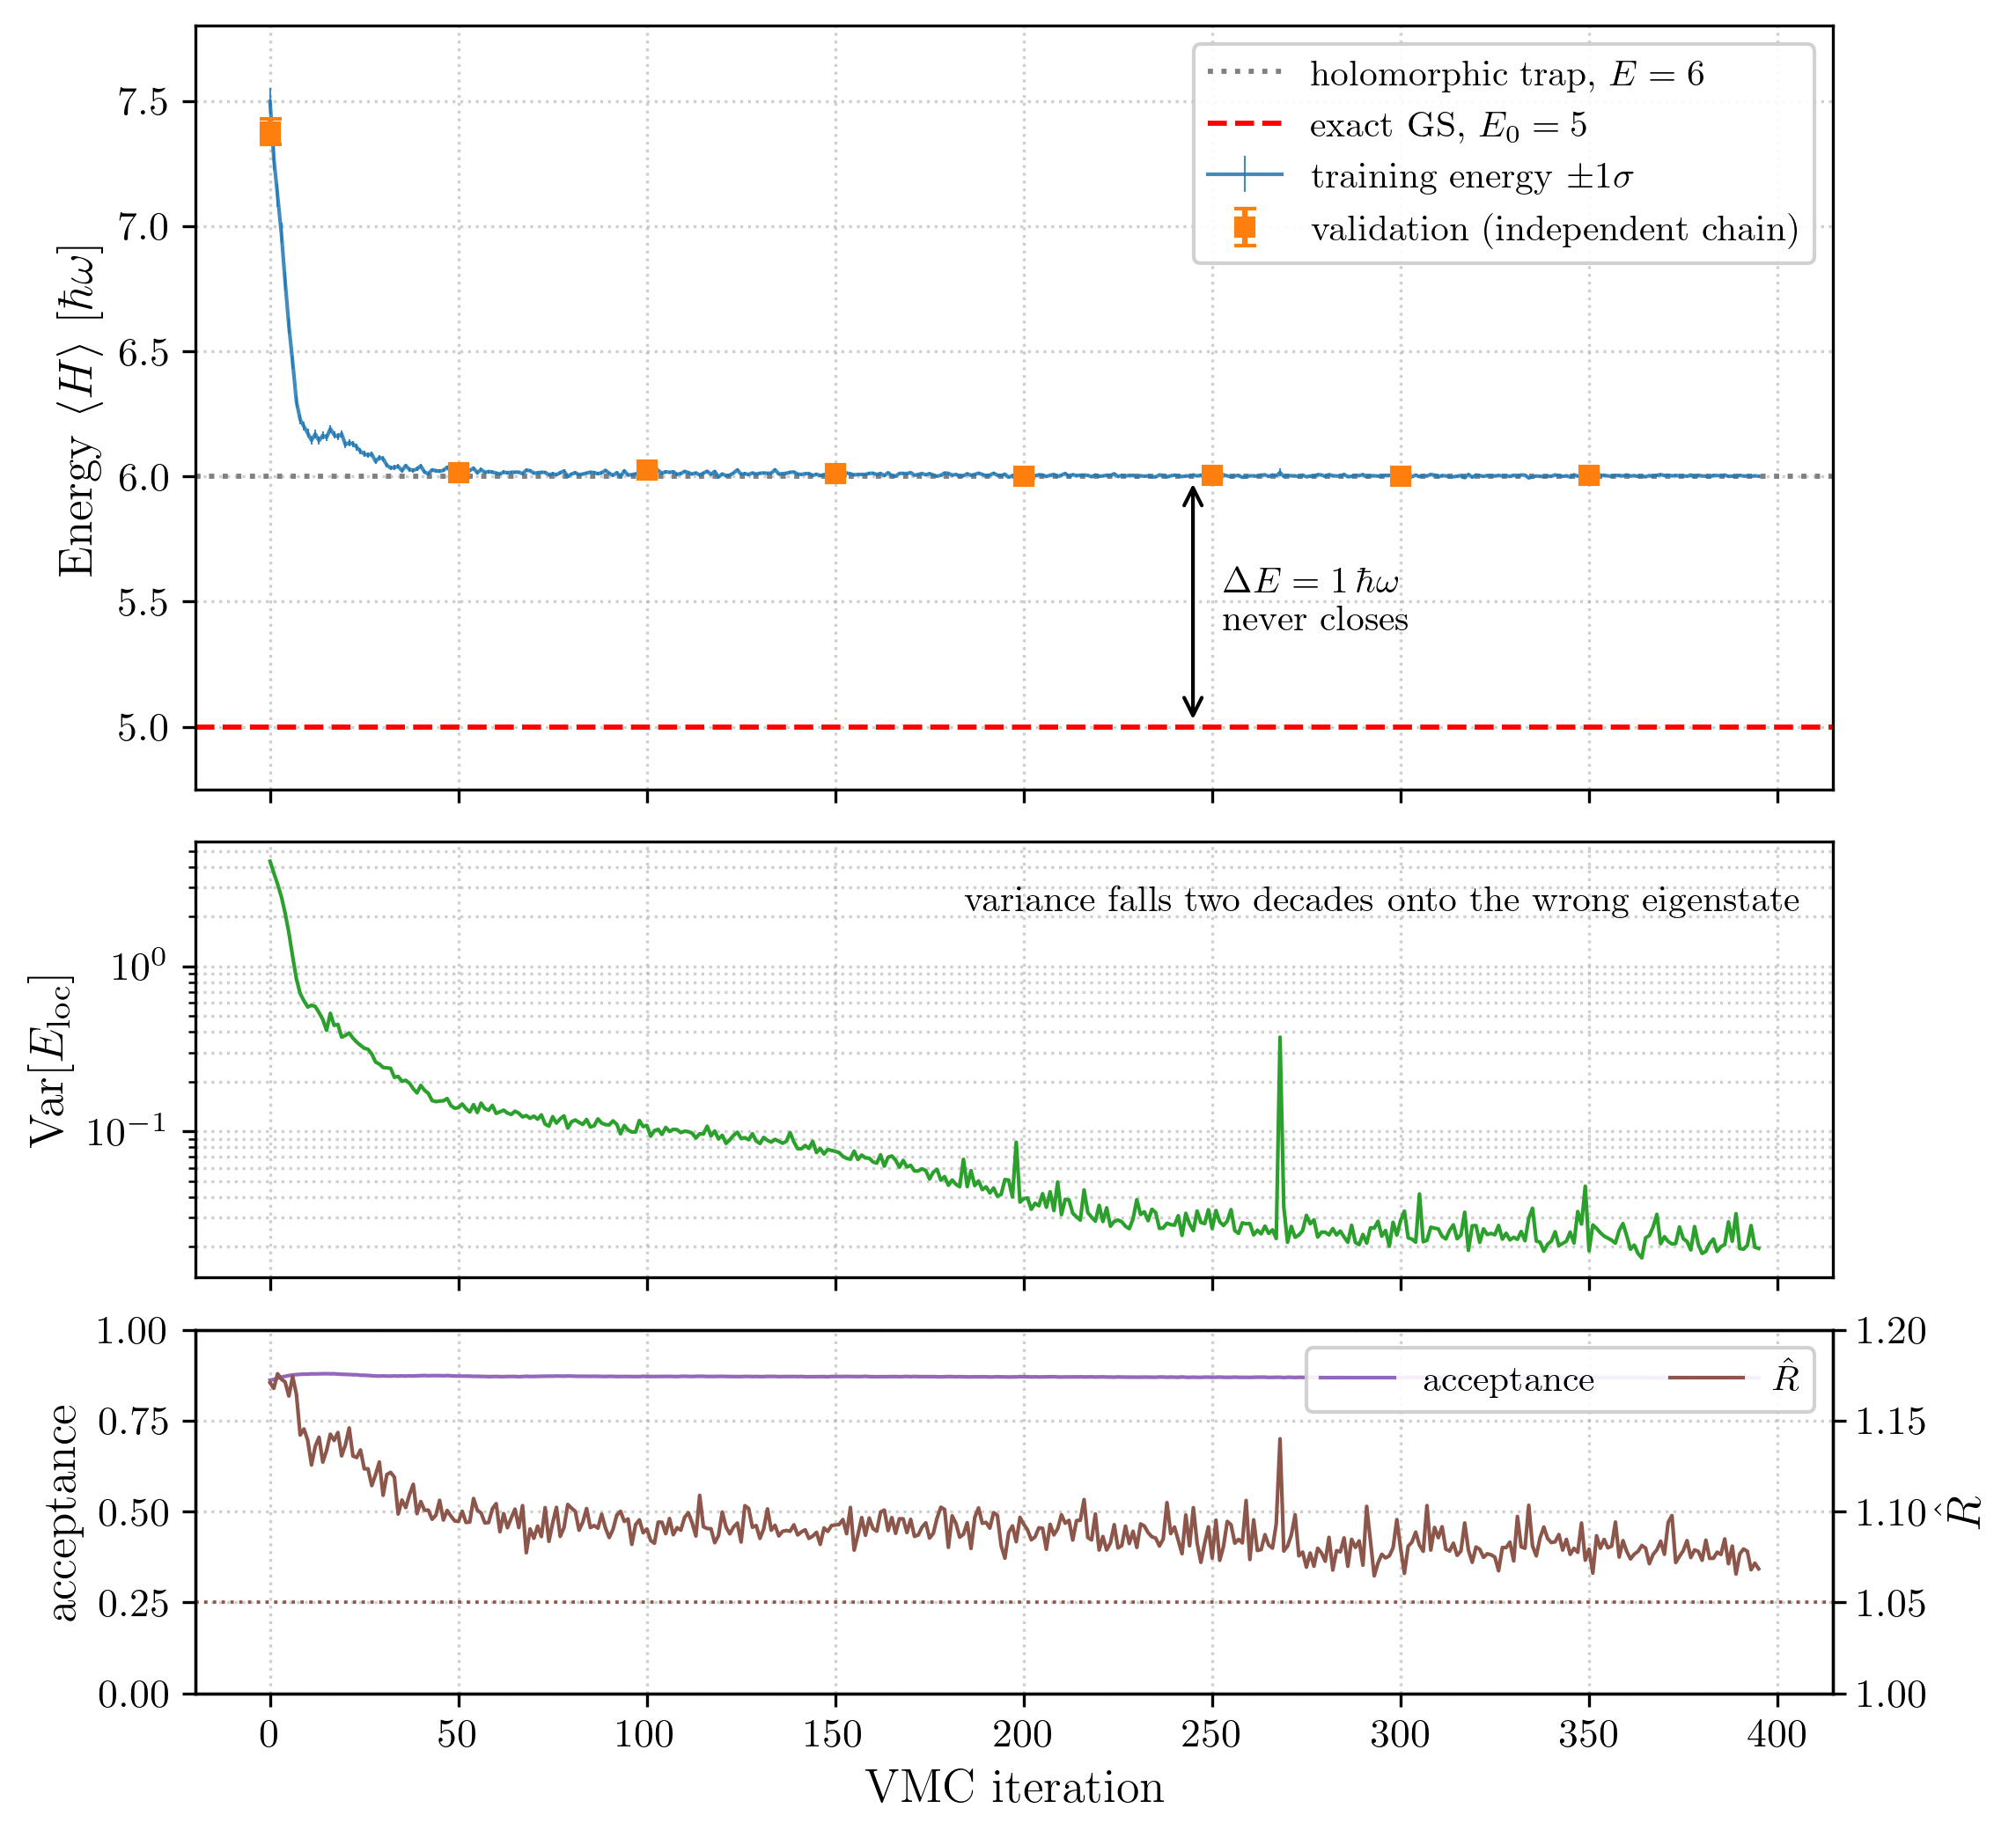
\includegraphics[width=1\linewidth]{n3_trap_convergence.png}
    \caption{from-scratch $N=3$ QHO run ($64$ hidden units, $4096$ samples, $512$ chains. Top: the training energy with its $1\sigma$ band and the independent-chain validation points, against the exact ground state $E_0 = 5$ and the holomorphic trap at $E = 6$; Middle: the variance of the local energy, falling two decades onto the trap. Bottom: sampler acceptance and $\hat R$.}
    \label{fig:n3_trap}
\end{figure}

For the visualisation purposes we pin two of the three particles at fixed positions and sweep the third over the plane, which turns the six-dimensional wavefunction into a 2D image, we can see the nodal structure. \ref{fig:n3_trap_walk} The two analytic candidates are distinguishable in this slice. The ground state $\det[1,x,y]$ vanishes whenever the three particles are collinear, so its node is an extended straight line running through both pinned particles and cutting the plane into two lobes. The holomorphic state vanishes only where the swept particle sits exactly on one of the other two, so it fails to recognise this "nodal line". 

Already at initialisation NN carries $\mathcal{F}_{\rm holo} = 0.42$, so the random network starts closer to the trap than to anything else, and within fifty iterations it has moved onto the crescent and stayed there, while its overlap with the ground-state panel never lifts off zero at any point in the run. The one feature of the late panels that the pure trap does not have, the dip breaking the crescent into two bright patches, is the $15\%$ of the weight that has drifted into the antiholomorphic mirror interfering with the holomorphic part. The mirror is not drawn, because it cannot be: it is the exact complex conjugate of the holomorphic state, so the two have identical densities at every configuration and differ only in phase, which is the reason the chirality has to be tracked through $\langle L_z\rangle$ in Section~\ref{sec:mirror_flip} rather than by looking at pictures.

\begin{figure}[H]
    \centering
    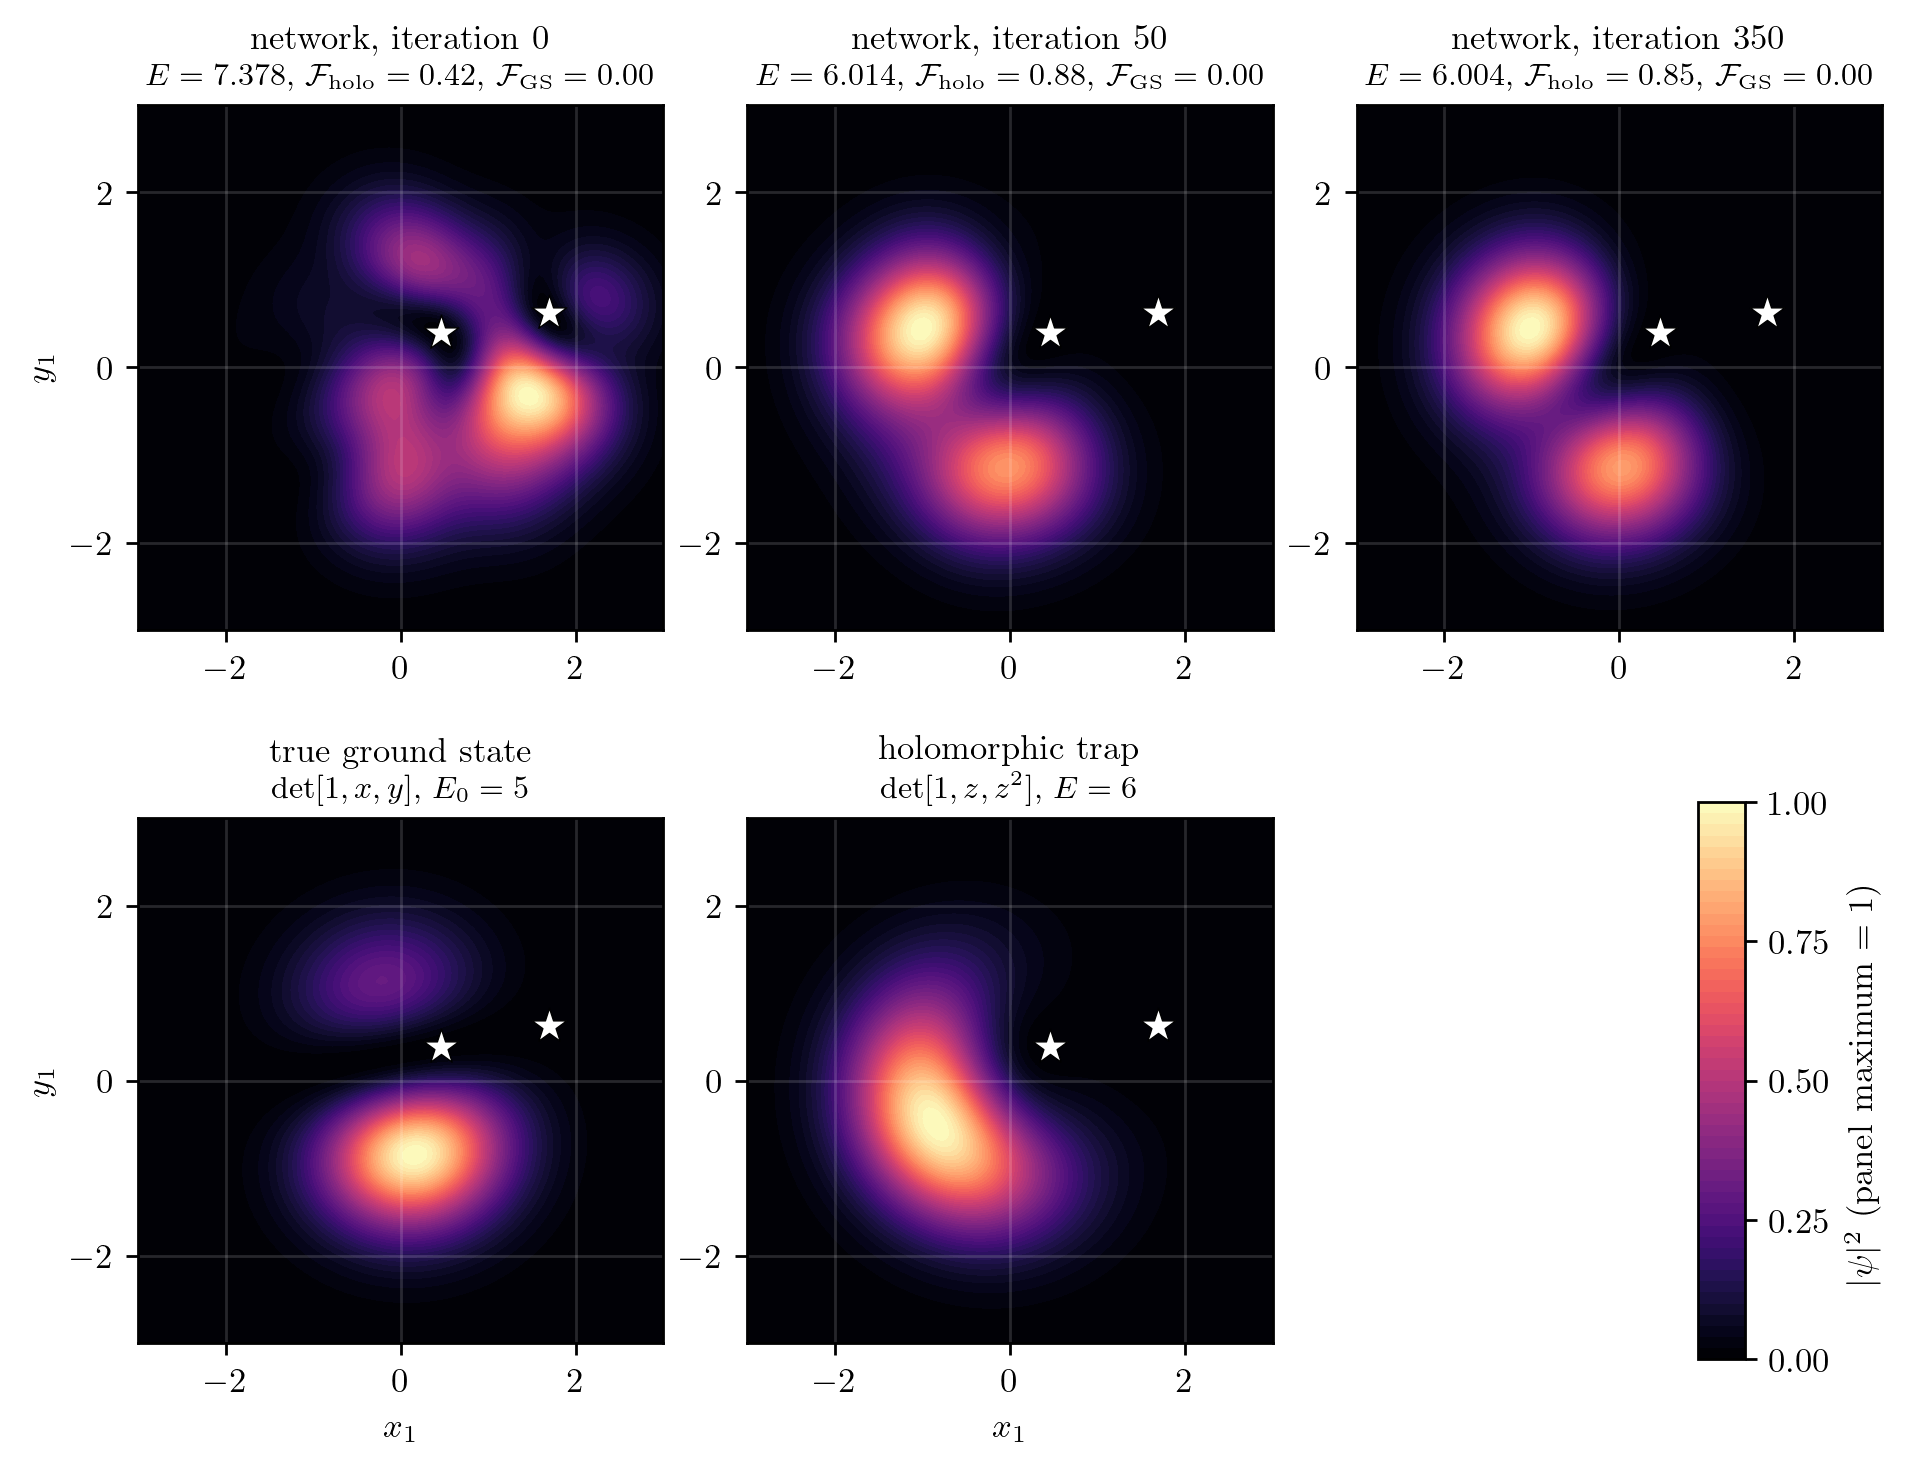
\includegraphics[width=1\linewidth]{n3_trap_density_walk.png}
    \caption{The walk into the trap, same run as Figure~\ref{fig:n3_trap}. Two particles are pinned (white stars) and the third is swept over the plane; each panel is normalised to its own maximum. Top: the network at iterations $0$, $50$ and $350$, annotated with the energy and the squared overlaps against the two analytic candidates. Bottom: the true ground state, whose collinearity node is an extended line through both pinned particles, and the holomorphic Vandermonde trap, whose only zeros are the two pinned positions. The network leaves initialisation already $42\%$ holomorphic, settles onto the crescent within fifty iterations, and never acquires any ground-state weight.}
    \label{fig:n3_trap_walk}
\end{figure}

\subsection{Adding a degenerate target: $N=4$}
\label{sec:n4}

To rule out some special situation, we repeat the experiment with four spinless fermions in the same trap, Equation~\ref{eq:hamiltonian} specialised to $N=4$. Here the ground state is no longer unique. From an analysis of the possible single-particle wavefunctions with $n = n_x + n_y$, the lowest shells and their $(n_x, n_y)$ states are

\begin{itemize}
    \item $n = 0$: $(0,0)$
    \item $n = 1$: $(0,1), (1,0)$
    \item $n = 2$: $(0,2), (2,0), (1,1)$
    \item $n = 3$: $(1,2), (2,1), (3,0), (0,3)$
\end{itemize}

Filling four fermions completes shells $n=0$ and $n=1$ and leaves the third shell ($n=2$, threefold degenerate) with a single occupant, so the true ground state is a threefold-degenerate combination of the form

\begin{equation}
\Psi_{\mathrm{GS}}
=
c_1\,\Psi_{2,0}
+
c_2\,\Psi_{1,1}
+
c_3\,\Psi_{0,2}
\end{equation}

and the Energy of this system would be : 
\begin{equation}
    E = \hbar \omega ( n_x + n_y + \frac{1}{2} + \frac{1}{2}) =  \hbar \omega  (( 0 + 0 + 1 ) + ( 0 + 1 + 1  )  +  ( 1 + 0 + 1  ) + ( 0 + 2 + 1  )) =  \hbar \omega 8
\end{equation}


The degeneracy turns out to change nothing about the failure. From the energy-convergence data (Figure~\ref{fig:n4_convergence}) we see same situation:  from a random start the network settles at $E = 10\,\hbar\omega = N(N+1)/2$, two full orbitals above the true ground state this time, and the smallest network never leaves it. The plateau is once more the holomorphic Vandermonde state of Section~\ref{sec:lazy_trap}, the two-dimensional analogue of the lowest-Landau-level Laughlin state $\Psi_{LL} = \text{Vandermonde}\cdot\text{Gaussian}$, and the fidelity (Equation~\ref{eq:fidelity}) against the analytic holomorphic determinant confirms it at $\mathcal{F} \approx 0.95$, with a further $0.05$ residing in the "antiholomorphic mirror". As established in Section~\ref{sec:lazy_trap}, the trap is not a single state but a degenerate mirror pair: the holomorphic state at $L_z = +N(N-1)/2$ and its complex conjugate, the antiholomorphic state at $L_z = -N(N-1)/2$, share the eigenvalue $E=10$.

\begin{figure}[H]
    \centering
    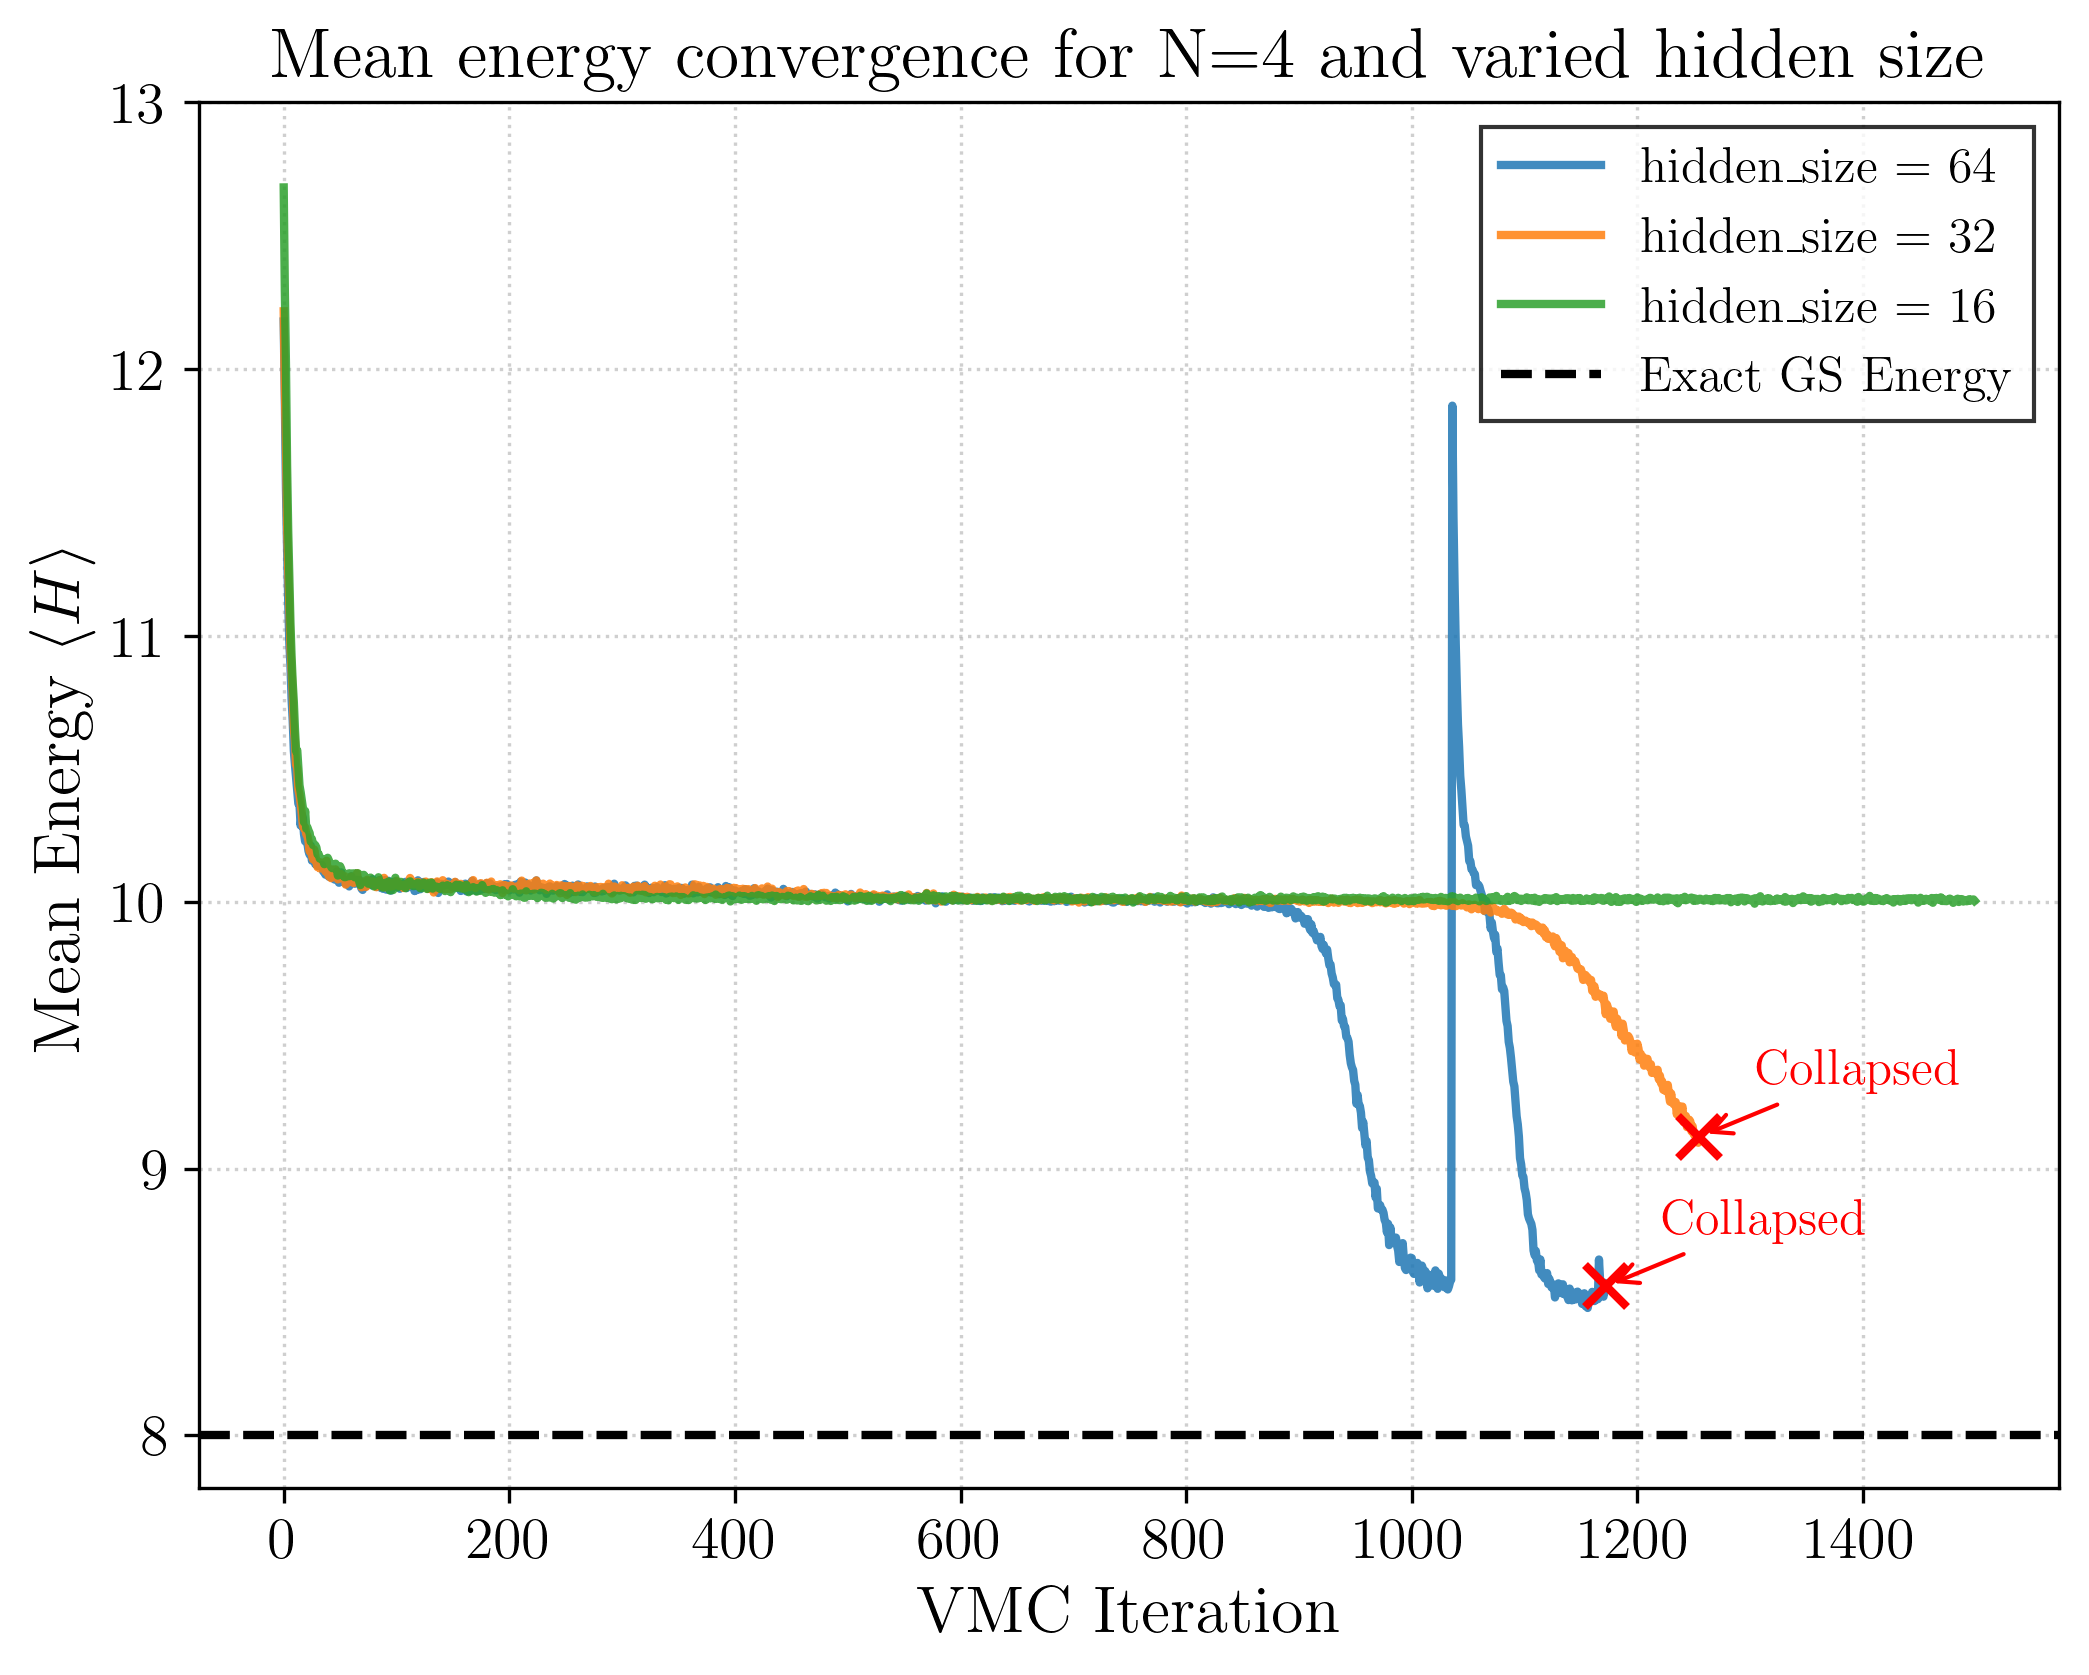
\includegraphics[width=15cm,height=10cm,keepaspectratio]{Mean_energy_convergence_for_N=4_and_varied_hidden_size.png}
    \caption{Energy convergence for the $N=4$ QHO ($E_0 = 8$, trap at $E = 10$) at hidden widths $16$, $32$, $64$. The $16$-unit run stays pinned on the trap for the entire run; the $32$- and $64$-unit runs leave it late in training, the $64$-unit reaching $E \approx 8.5$ before a stochastic-reconfiguration instability collapses the run. No width reaches the true ground state.}
    \label{fig:n4_convergence}
\end{figure}

\subsection{Brute force with more capacity}
\label{sec:brute_force}

As we see at the convergence graph \ref{fig:n4_convergence} the capacity of the network helped with escaping the trap to some extend.

The first hypothesis we could make is that the trap is a failure of expressivity, that a wider network would simply represent the ground state and descend to it. Width alone does not settle that question either way, as the scan below shows and as Section~\ref{sec:pretraining} then explains. Figure~\ref{fig:n4_convergence} already shows the first sign: at $16$ hidden units the energy sits exactly on the trap for the whole run, but at $32$ and $64$ units the network does begin to leave it, dropping below $E=10$ late in training, with the $64$-unit run reaching as low as $E \approx 8.5$ before the update becomes unstable and the run collapses.

So capacity does something, and we pushed to the limit of the hardware. Table~\ref{tab:width_scaling} collects, for every hidden width we ran (from $16$ up to $512$, the largest sized to fill an $80$\,GB GPU), the deepest energy reached that stayed physically valid and stable, together with how many runs at that width stayed trapped, collapsed through a stochastic-reconfiguration instability, or escaped the trap and held a lower energy.

\begin{table}[H]
    \centering
    \begin{tabular}{r r r r r c}
        \hline
        hidden & runs & trapped & collapsed & escaped \& held & record stable $E$ \\
        \hline
        16  & 2  & 2  & 0  & 0  & $10.0$ (trap) \\
        32  & 3  & 1  & 2  & 0  & $-$ \\
        64  & 46 & 29 & 5  & 12 & $\mathbf{8.36}$ \\
        128 & 3  & 1  & 2  & 0  & $-$ \\
        256 & 17 & 5  & 11 & 1  & $8.71$ \\
        300 & 4  & 3  & 1  & 0  & $10.1$ (trap) \\
        512 & 1  & 1  & 0  & 0  & $9.6$ \\
        \hline
    \end{tabular}
    \caption{Hidden-width scaling for the $N=4$ QHO trap ($E_0 = 8$, trap at $E = 10$), across all $76$ from-scratch runs. ``Escaped \& held'' counts runs that dropped below the trap and stayed there without collapsing; ``record stable $E$'' is the lowest such energy (``$-$'' where no run escaped stably). No width, up to $512$ units on $80$\,GB, reaches the true ground state.}
    \label{tab:width_scaling}
\end{table}

From empirical testing we get following : 
\begin{itemize}
    \item Capacity breaks the trap, but does not converge. The record energy improves from $9.99$ at $16$ units to $8.36$ at $64$ units, yet no width reaches the true ground state $E_0 = 8$; the best stable result across all $76$ runs is $E \approx 8.3$, a relative error of roughly $4\%$.
    \item Beyond $64$ units, more hidden units makes things worse. The larger networks ($128$ to $512$) cause stochastic-reconfiguration to collapse.
    \item The escape is fragile even at its best width: only about a quarter of the $64$-unit runs escape and hold, the rest stay trapped or collapse. The record result was achieved by sheer lack and meticulous tuning of training parameters \ref{app:ablations}
\end{itemize}

A larger network can bend partially the trap, but it cannot reach the ground state and it destabilises the optimiser in the attempt. However we can't eliminate the question of Ansatz expressivity yet so we will return to in in Section~\ref{sec:pretraining}.

\subsection{Supervised pretraining}
\label{sec:pretraining}

Definitive test confirming trainability/expressivity question is supervised pretraining. And running a bit ahead of time, we wish we did these experiments much earlier in our work. Instead of minimising the energy, we give the network the answer and ask it to imitate it: we fit $\log\psi_{\theta}$ to the analytic ground state by gradient descent on a supervised loss, drawing configurations from a broad Gaussian and matching both the log and the phase of the target,
\begin{equation}
    \mathcal{L}(\theta) = \underbrace{\mathrm{Var}_x\!\big[\mathrm{Re}(\log\psi_\theta - \log\psi_{\mathrm{GS}})\big]}_{\text{amplitude}} \; + \; \underbrace{\big\langle 1 - \cos\mathrm{Im}(\log\psi_\theta - \log\psi_{\mathrm{GS}})\big\rangle}_{\text{phase}},
    \label{eq:supervised_loss}
\end{equation}
The target is the exact non-interacting ground state, which for the harmonic trap is a single Slater determinant of oscillator orbitals. If the ansatz can be driven onto the ground state this way the state is representable, and that direction is a constructive proof. The converse is weaker proof (TODO: literature check with \cite{wu_supervised_2024} etc) What the test does deliver is an upper bound on what is achievable in practice, since it removes the Monte Carlo noise and the variational energy landscape and hands the network the answer outright. We therefore read a stalled fit as strong evidence against the representability and strengthen it by closing the remaining optimization explanations one at a time.

For the closed-shell benchmark at $N=3$ this test converges well towards ground state. The supervised loss falls, the phase term reaches $0.19$, and when we release ordinary VMC from the pretrained parameters the energy settles onto the true ground state at $E \approx 5.05$ with fidelity $\mathcal{F} \approx 0.99$ against the analytic determinant, instead of drifting back up to the trap at $E=6$. The network is therefore fully capable of representing the $N=3$ ground state; what it lacks from a real scenario is initialisation with any gradient that leads there. 

Later we found the same does not hold for larger systems. We therefore ran the identical fit at every particle number we study. Two of them need care: $N=4$ and $N=5$ are open shells, so the ground state is degenerate and NN picks one orbital arbitrarily. We fit two distinct orbitals at each.



\begin{figure}[H]
    \centering
    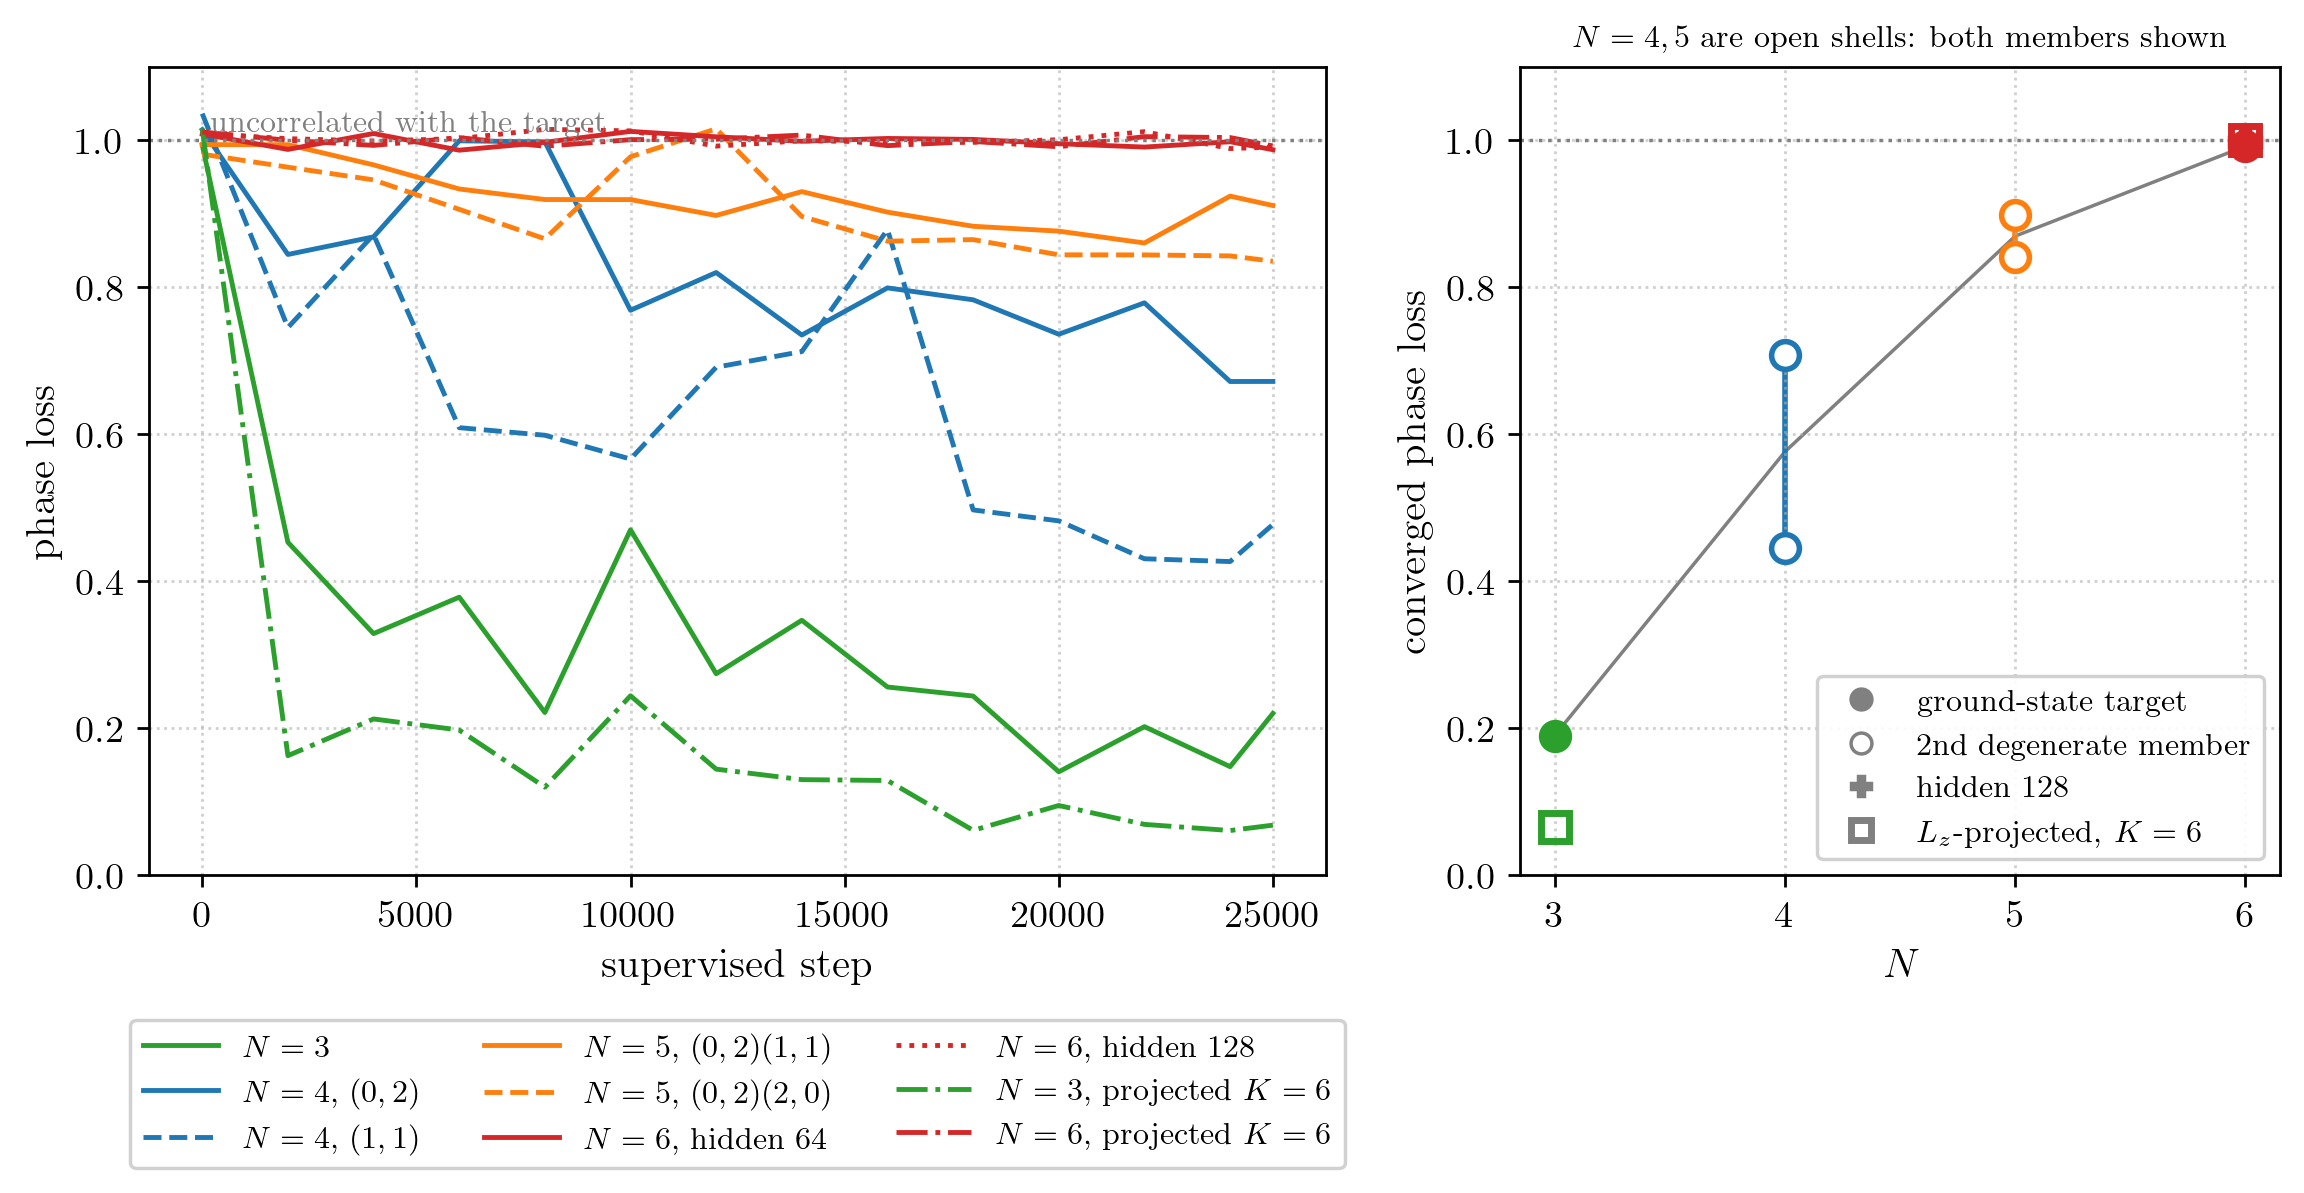
\includegraphics[width=1\linewidth]{supervised_assay.png}
    \caption{Supervised expressivity ablation across particle number Left: phase loss against supervised step Right: the converged phase loss against $N$, open circles marking the second member of the degenerate ground-state at the open shells $N=4$ and $N=5$, and the cross marking $N=6$ at hidden $128$. The degradation is monotone in $N$, the member choice shifts the value but not the trend, and width is not a lever.}
    \label{fig:supervised_assay}
\end{figure}

The result is in Table~\ref{tab:supervised} and Figure~\ref{fig:supervised_assay}. Alongside the two loss terms we report the squared overlap $\mathcal{F}$ of each fitted state with its target, and it is the overlap that should be read: it is an observable, and it weights configurations by $|\psi|^2$, whereas the phase term weights every configuration's angle equally and so overstates the failure wherever the state carries little probability. Read that way the division is sharp. At $N=3$ the ansatz reproduces the ground state ($\mathcal{F} = 0.91$) and at $N=4$ it still captures most of it ($0.80$), at $N=5$ only a tenth remains ($0.11$), and from $N=6$ through $N=8$ the overlap is numerically zero. The failure is not an accident of how the fits were run, and we closed each way it could have been one. It is not the optimisation budget, since quadrupling it moves $N=4$ only from $0.71$ to $0.59$, nowhere near the $0.19$ that constitutes a fit at $N=3$, and leaves $N=6$ at $0.995$. It is not decoder capacity, since doubling the hidden width at $N=6$ changes nothing. It is not the random seed: three seeds give $1.000 \pm 0.009$ at $N=6$ and $0.478 \pm 0.052$ at $N=4$, so the ceiling reproduces to about one percent. It is not the arbitrary choice of degenerate member, since both members fail at both open shells. What survives all of this is a single ordering. The overlap tracks how many shell-$2$ orbitals the target occupies, those being the ones whose nodal structure is not holomorphic, falling from $0.91$ with none of them to $0.80$, $0.11$ and $0$ as one, two and three are filled. The spread within $N=4$ reads the same way, since shell $2$ carries $m \in \{-2,0,+2\}$ and $(1,1) \propto xy$ is pure $|m| = 2$ while $(0,2) \propto y^2$ mixes in $m = 0$, and a holomorphic $\eta$ favours maximal $|m|$.

\begin{table}[H]
    \centering
    \begin{tabular}{l l r r r}
        \hline
        system & shell-$2$ orbitals & amplitude & phase & $\mathcal{F}$ \\
        \hline
        $N=3$, closed shell & $-$              & $0.38$ & $0.19$ & $\mathbf{0.911}$ \\
        $N=4$               & $(1,1)$          & $0.68$ & $0.45$ & $\mathbf{0.799}$ \\
        $N=4$               & $(0,2)$          & $0.75$ & $0.71$ & $0.297$ \\
        $N=5$               & $(0,2)\,(2,0)$   & $0.92$ & $0.84$ & $0.109$ \\
        $N=5$               & $(0,2)\,(1,1)$   & $0.93$ & $0.90$ & $0.026$ \\
        $N=6$, closed shell & all three        & $1.07$ & $0.99$ & $\mathbf{0.0000}$ \\
        $N=7$               & all three $+$ shell $3$ & $1.23$ & $1.01$ & $0.0000$ \\
        $N=8$               & all three $+$ shell $3$ & $1.50$ & $1.00$ & $0.0001$ \\
        \hline
        \multicolumn{5}{l}{\emph{controls: none of them changes the outcome}} \\
        $N=6$, hidden $128$          & all three & $0.99$ & $0.99$ & $0.0001$ \\
        $N=4$ $(1,1)$, $100{,}000$ steps & $(1,1)$ & $0.72$ & $0.53$ & $0.731$ \\
        $N=6$, $100{,}000$ steps     & all three & $1.19$ & $0.995$ & $0.0000$ \\
        $N=3$, $L_z$-projected $K=6$ & $-$       & $0.16$ & $0.07$ & $\mathbf{0.995}$ \\
        $N=6$, $L_z$-projected $K=6$ & all three & $1.05$ & $0.99$ & $ 0.0001$ \\
        \hline
    \end{tabular}
    \caption{Supervised fit of the FermiSets ansatz to the exact non-interacting ground state (Equation~\ref{eq:supervised_loss}, hidden $64$ and $25{,}000$ steps unless stated; loss terms are means over the last three logged points). The phase term runs from $0$, sign structure matched, to $1$, uncorrelated. $\mathcal{F} = |\langle\psi_{\mathrm{fit}}|\psi_{\mathrm{GS}}\rangle|^2$ is estimated by importance sampling from $\mathcal{N}(0,1)^{N\times 2}$ with $2\times10^5$ samples, bootstrap error below $0.005$ throughout. At the open shells $N=4$ and $N=5$ the ground state is degenerate and each is fitted against two distinct members. The $N=6$ projected overlap is absent because that run's checkpoint was lost to an out-of-memory failure in the post-fit evaluation, which does not affect its loss terms. We omit the VMC energy of the fitted states: the masked loss ignores the near-collision region that VMC samples in full, so those energies carry $\sigma^2$ between $10^3$ and $10^{11}$ and measure nothing.}
    \label{tab:supervised}
\end{table}

\newpage

\subsection{Angular momentum in the 2D QHO}
\label{sec:angular_momentum}

In two dimensions the trap is rotationally symmetric, so alongside the energy each single-particle level carries a definite angular momentum, which allows us to expoit symmetry of the system and another good quatum number : $m$. The same shell $n = n_x + n_y$ can be relabelled by a radial quantum number $n_r$ and a magnetic quantum number $m$ through
\begin{equation}
    E = \hbar\omega\,(n + 1) = \hbar\omega\,(n_x + n_y + 1) = \hbar\omega\,(2 n_r + |m| + 1),
\end{equation}
where $m$ is the eigenvalue of the angular-momentum operator
\begin{equation}
    \hat L_z = -i\hbar\,(x\,\partial_y - y\,\partial_x) = \hbar\,(z\,\partial_z - \bar z\,\partial_{\bar z}).
    \label{eq:lz_operator}
\end{equation}
Within a shell of index $k$ the allowed magnetic numbers run in steps of two from $-k$ to $+k$, so the shells resolve into definite-$L_z$ states as

\begin{itemize}
    \item $k=0$ ($E=1$): $m = 0$
    \item $k=1$ ($E=2$): $m = -1, +1$
    \item $k=2$ ($E=3$): $m = -2, 0, +2$
    \item $k=3$ ($E=4$): $m = -3, -1, +1, +3$
\end{itemize}

For a many-body state the total angular momentum is additive, $L_z^{\text{tot}} = \sum_i m_i$, and is conserved because $[\hat H, \hat L_z^{\text{tot}}] = 0$. Filling the closed shells for $N=3$ gives $L_z = 0$; the holomorphic trap of Section~\ref{sec:lazy_trap}, which fills the maximal-$m$ orbital of each shell, instead carries $L_z = \sum_{k=0}^{N-1} k = N(N-1)/2$. This difference in angular momentum between the ground state and the trap is exactly the handle the projection in Section~\ref{sec:lz_projection} uses.

\subsection{Escaping the trap by symmetry projection}
\label{sec:lz_projection}

The theory of Section~\ref{sec:lazy_trap} points to a structural remedy that needs no prior knowledge of the ground state. The trap is a pair of states carrying nonzero angular momentum, $L_z = \pm N(N-1)/2$, while the ground state of a rotationally symmetric, closed-shell system carries $L_z = 0$. If we can force the ansatz into the $L_z = 0$ sector, the trap is simply not in the space it is allowed to explore.

Because the isotropic trap satisfies $[\hat H, \hat L_z] = 0$, its eigenstates can be chosen as eigenstates of $\hat L_z$, and we project onto a definite sector by averaging the symmetric part of the network over $K$ equally spaced rotations,
\begin{equation}
    \xi(R) \;\longmapsto\; \frac{1}{K}\sum_{k=0}^{K-1} \xi\big(R_{\theta_k}\big), \qquad \theta_k = \frac{2\pi k}{K},
    \label{eq:lz_projection}
\end{equation}
applied to the coordinates fed into the symmetric branch. A component of angular momentum $m$ picks up a phase $e^{im\theta}$ under rotation, so the $K$-fold average annihilates every component except those with $L_z \equiv 0 \pmod K$: the ground state ($m=0$) survives, and the trap pair ($m = \pm N(N-1)/2$) is removed whenever $N(N-1)/2 \not\equiv 0 \pmod K$. The cost is a factor of $K$ in the forward pass, so the ansatz scales as $O(K\,N^2)$ against the $O(N^3)$ of a Slater determinant.

At $N=3$ this works, and it is our first success. The trap sits at $L_z = \pm 3$, so any $K$ not dividing $3$ removes it. From a random start the projected network converges to the true ground state, $E = 5.015 \pm 0.004$ against the exact $E_0 = 5$, with fidelity $\mathcal{F} = 0.9988$ against the analytic ground-state determinant (Figure~\ref{fig:lz_n3_qho}). Evaluated without the projection, the very same trained parameters give $E = 7.41$ and negligible ground-state weight, confirming that it is the projection, not the network alone, that selects the physical state. The same construction solves the interacting quantum dot of Section~\ref{impl:sys}: with $K=6$ the network reaches $E = 6.212$ against the exact-diagonalisation value $6.2107$, a relative error of $0.09\%$ (Figure~\ref{fig:lz_n3_dot}), whereas the unprojected run parks on the interaction-deformed trap at $E = 7.02$.

\begin{figure}[H]
    \centering
    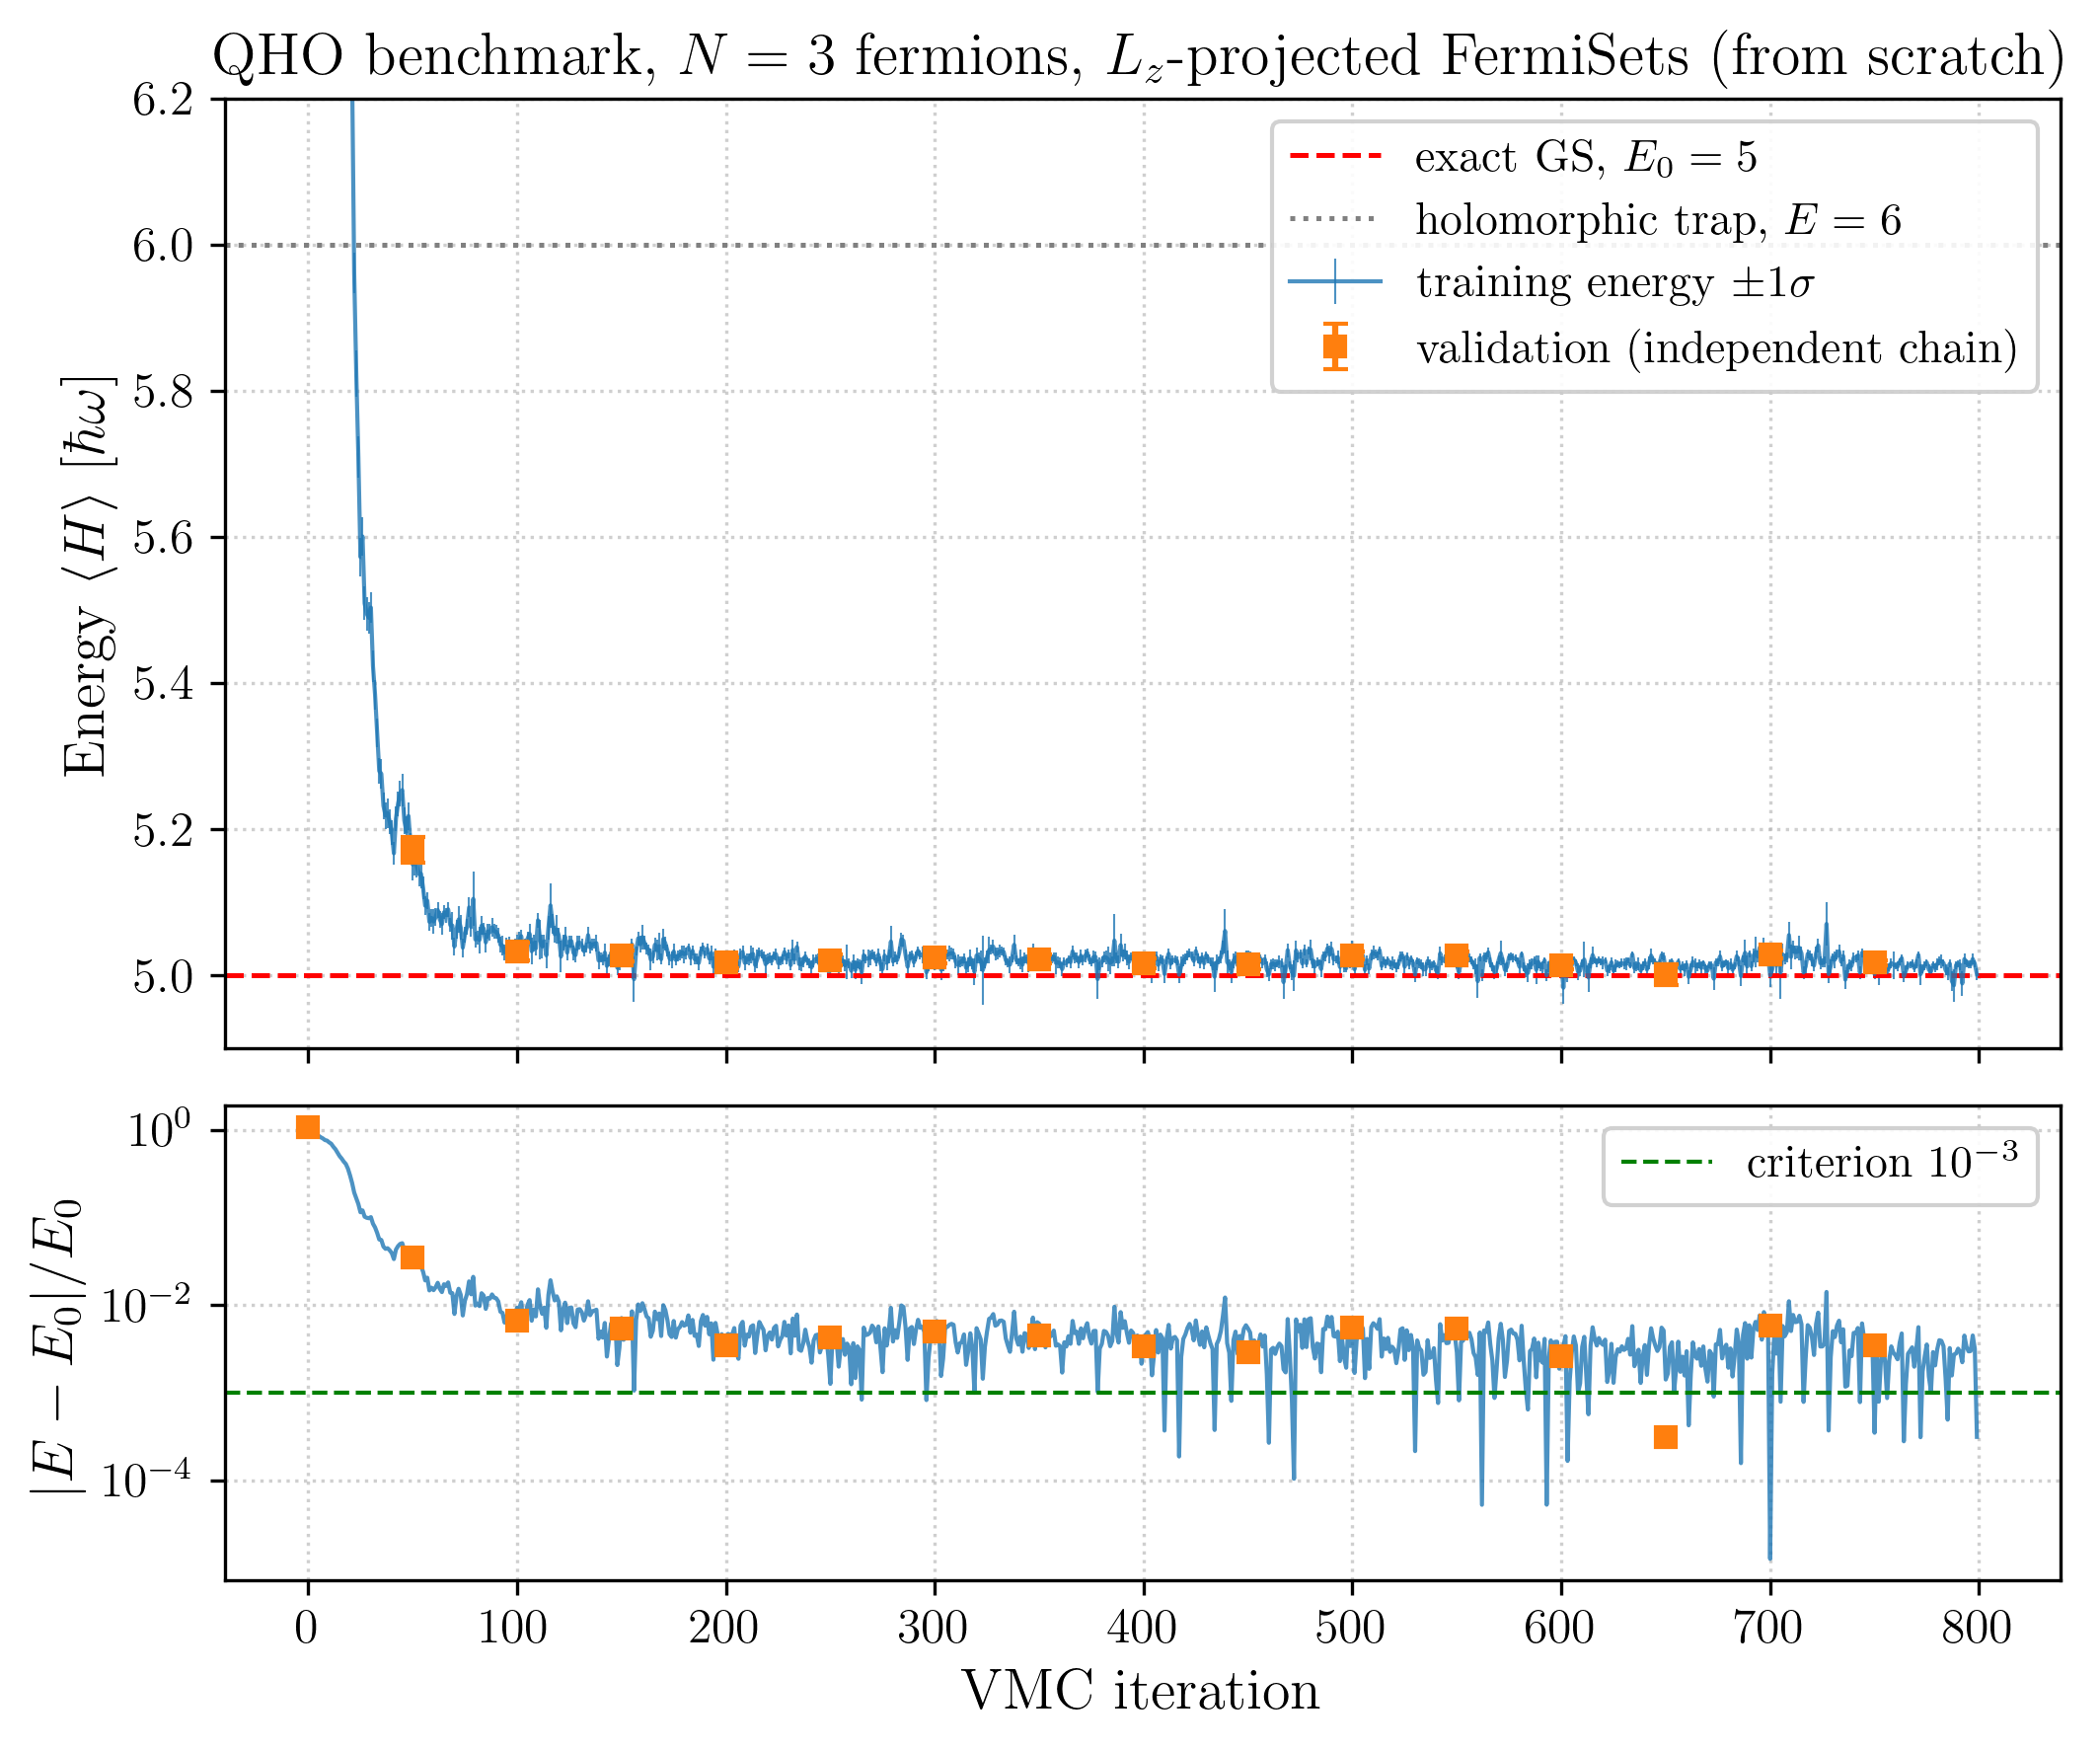
\includegraphics[width=0.8\linewidth]{qho_lz_N3_convergence_pub.png}
    \caption{$N=3$ QHO with $L_z$ projection: energy and relative error against the exact ground state $E_0 = 5$. The independent-chain validation energy tracks the training energy, and the run converges to $\sim 0.2\%$, escaping the trap at $E=6$ (dotted).}
    \label{fig:lz_n3_qho}
\end{figure}

Read against the trap, the effect of the projection is best seen in the same slice as before. Figure~\ref{fig:lz_n3_walk} repeats Figure~\ref{fig:n3_trap_walk} for the projected run, at identical seed, architecture and hyperparameters, the only difference being $K=6$ instead of no projection. The starting point is not the near-trap configuration of before but a scrambled multi-lobe density with no weight on either candidate, since the sieve annihilates most of what the random network happens to contain. From there the walk goes the other way: by iteration $50$ the density has acquired the collinearity node of the ground state and $\mathcal{F}_{\rm GS} = 0.97$, and by iteration $750$ it is visually indistinguishable from the analytic ground-state panel at $\mathcal{F}_{\rm GS} = 0.999$, with the holomorphic and antiholomorphic overlaps held at $10^{-5}$ throughout. The two figures together are the cleanest statement of the result: the same optimiser on the same architecture walks into the trap or into the ground state depending only on which angular-momentum sector it is allowed to occupy.

\begin{figure}[H]
    \centering
    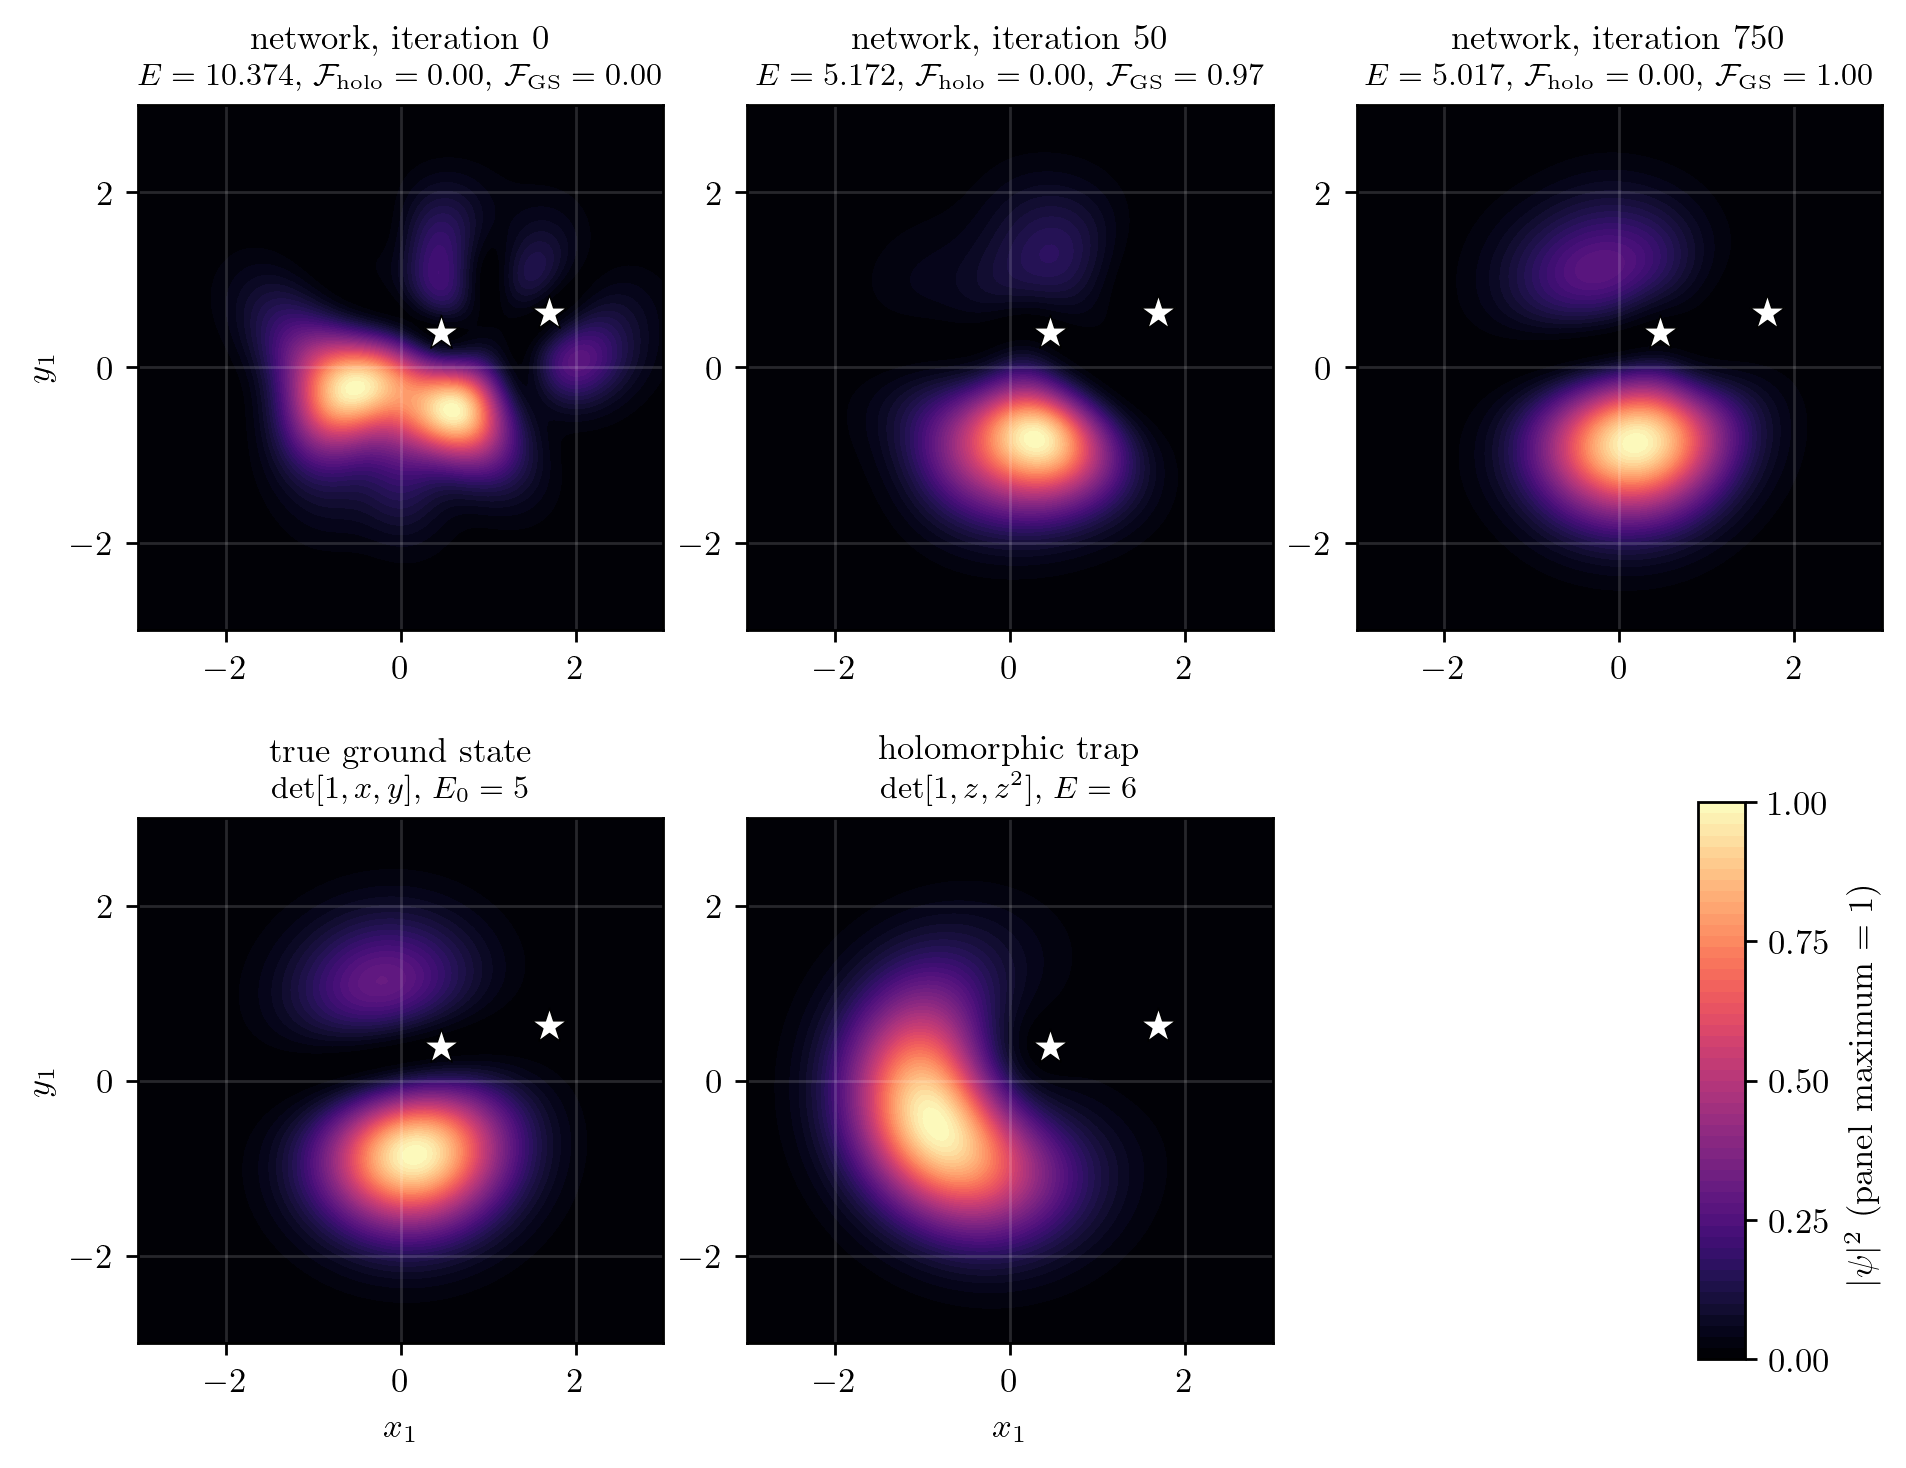
\includegraphics[width=0.75\linewidth]{n3_lz_density_walk.png}
    \caption{The same construction as Figure~\ref{fig:n3_trap_walk} for the $L_z$-projected run }
    \label{fig:lz_n3_walk}
\end{figure}

\begin{figure}[H]
    \centering
    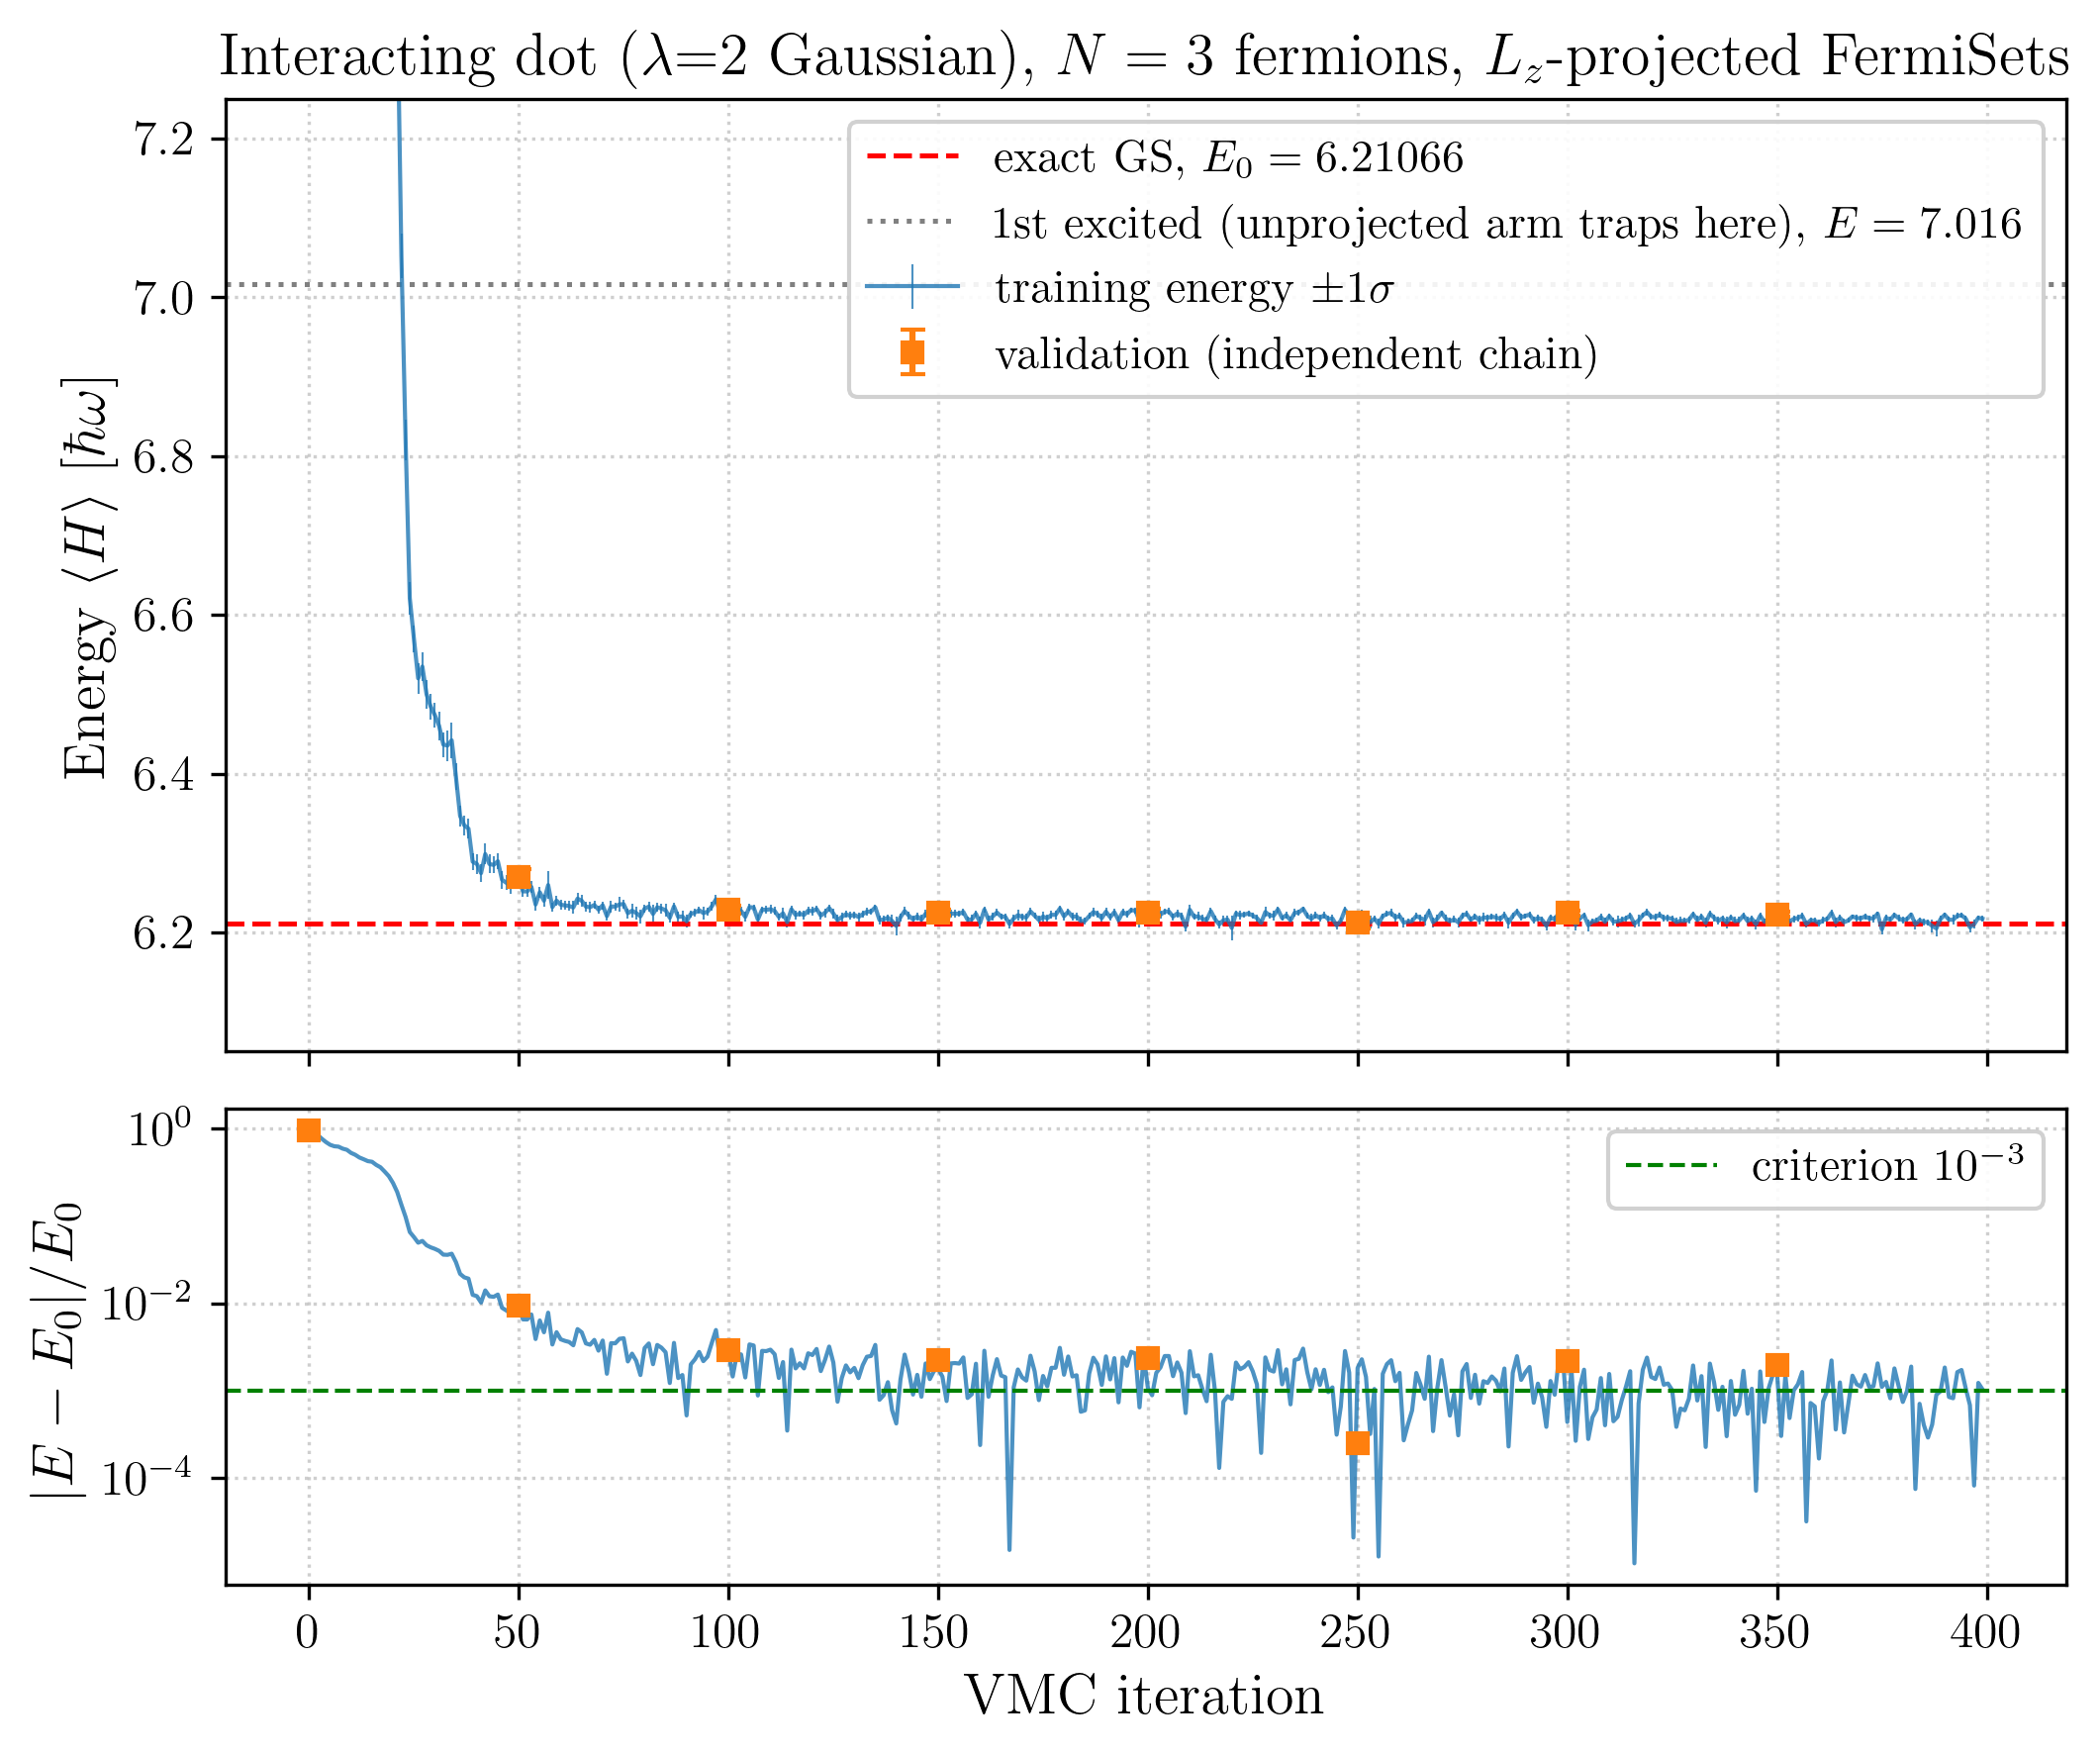
\includegraphics[width=0.8\linewidth]{dot_gauss_lz_N3_convergence_pub.png}
    \caption{$N=3$ interacting quantum dot with $L_z$ projection ($K=6$): convergence to the exact-diagonalisation ground state at $0.09\%$ relative error, demonstrating that the projection remedy is not specific to the non-interacting trap.}
    \label{fig:lz_n3_dot}
\end{figure}

\newpage

\subsubsection{Why the escape does not scale: N=6}
\label{sec:n6_wall}

The projection removes the trap, but it does not make the ansatz a general-purpose ground-state solver. At $N=6$ (the next closed shell, $E_0 = 14$, trap at $E = 21$) the projected network no longer reaches the ground state. Across $K = 3, 4, 6$ it descends below the trap but stalls at $E \approx 16$ to $17$, well short of $14$, and slower than the Slater-determinant baseline; at $N=10$ the stochastic-reconfiguration update diverges outright.


\begin{figure}[H]
    \centering
    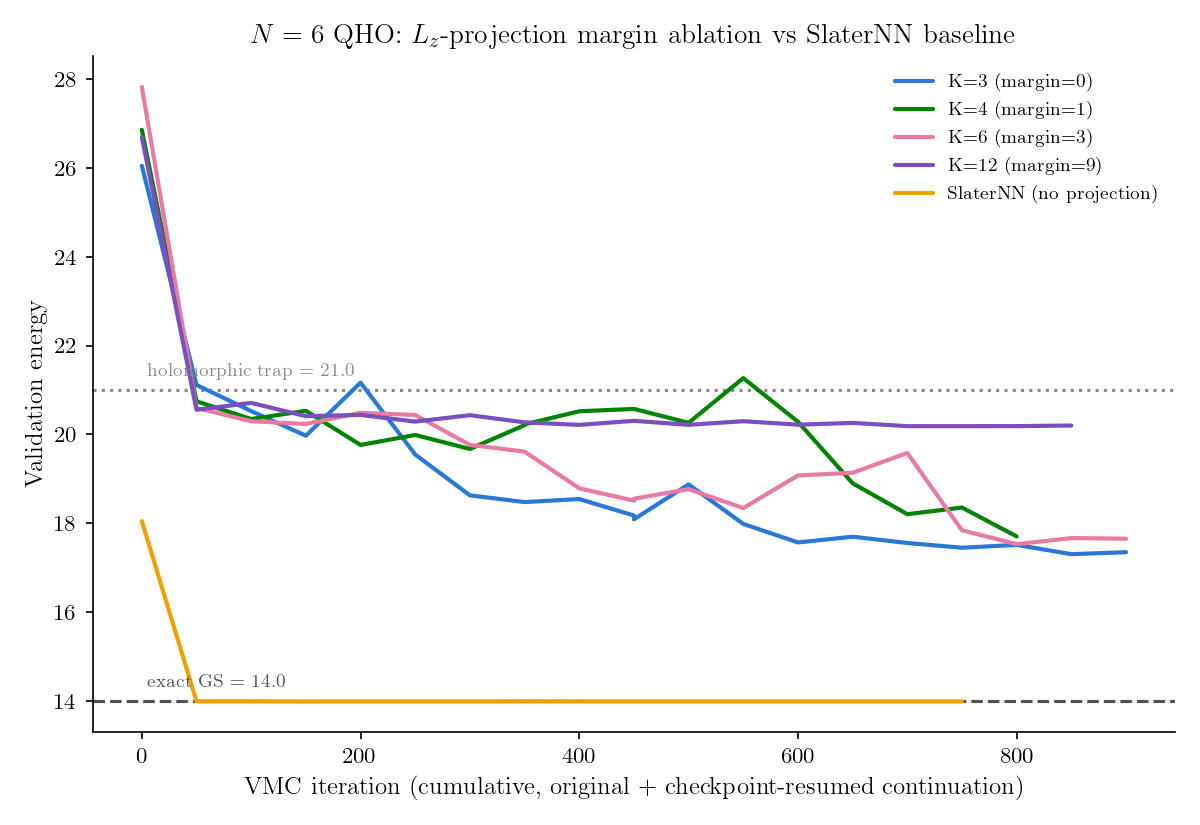
\includegraphics[width=0.9\linewidth]{n6_margin_ablation_vs_slater.png}
    \caption{$N=6$ QHO ($E_0 = 14$, trap at $E=21$). Projected FermiSets at $K=3,4,6$ all descend below the trap but stall together in the $E \approx 16$ to $17$ band,  independently of the projection order, while the Slater-determinant baseline of Section~\ref{sec:slaternn} drops cleanly to the ground state within a few tens of iterations. That the three projection orders track one another, even though $K=3$ leaves the trap inside the allowed sector while $K=6$ removes it, is the first sign that the plateau is not the trap but a same-sector obstruction the projection cannot reach.}
    \label{fig:n6_margin}
\end{figure}

The important point is that this is a different failure from the trap, and the projection is powerless against it. We must note there is no eigenstate at $E \approx 17$ in the $L_z = 0$ sector at all. Counting the non-interacting many-body states of $N=6$ with total $L_z = 0$ gives the ladder in Table below: the ground state is isolated at $E = 14$, and the first excited states appear only at $E = 16$ and $E = 18$, with the number of states exploding as the energy rises. A stable estimate at $17.4$ is therefore not a single eigenstate but a superposition sitting between the $E=16$ and $E=18$ eigenstates, which is consistent with the modest ground-state overlap measured on the plateau.

\begin{table}[t]
  \centering
  \caption{Low-lying non-interacting spectrum of $N=6$ in the
  $L_z = 0$ sector. Odd energies contain no $L_z = 0$ state, since a
  single shell hop flips the parity of the magnetic quantum number and
  $L_z \equiv E - N \pmod 2$; those levels are omitted. The ground
  state is an isolated needle beneath an exponentially growing set of
  excited levels. Energies in units of $\hbar\omega$.}
  \label{tab:n6_lz0_counting}
  \begin{tabular}{ccl}
    \toprule
    $E$ & $\#\{L_z = 0\}$ & \\
    \midrule
    14 & 1   & ground state, isolated \\
    16 & 9   & first excited level \\
    18 & 64  & second excited level \\
    20 & 255 & \\
    \bottomrule
  \end{tabular}
\end{table}

These excited states share the ground state's angular momentum, $L_z = 0$, so they lie in the exact sector the projection is designed to keep. No choice of $K$ can remove them: symmetry projection separates states of different symmetry, and here the obstruction has the same symmetry as the target. This is confirmed directly by the projection itself. At $N=6$ the trap sits at $L_z = \pm 15$; the choice $K=3$ leaves it untouched (since $15 \equiv 0 \pmod 3$) while $K=6$ removes it, yet both plateau at the same $E \approx 16$ to $17$. If the plateau were the trap, removing it would change where the network lands. It does not, because the plateau is built from same-sector excited states, not from the trap.

That this is a wall of representability, and not of optimisation budget or network width, is what the supervised assay of Section~\ref{sec:pretraining} already showed: at $N=6$ the amplitude term improves while the phase term never leaves $1$, at both $64$ and $128$ hidden units, and it is the only system in the study where the fit does not move at all (Figure~\ref{fig:supervised_assay}). Doubling the width changes nothing, because width buys decoder capacity and the missing ingredient is not decoder capacity: it is nodal freedom.


\subsubsection{Oscillation between the mirror states}
\label{sec:mirror_flip}

Now this section will briefly attempt to explain what happened in the runs where huge networks were lucky to escape the trap. We made a short movie to see how the function evolves over time and seen the network oscillating the "petals" of wavefunction projection between to chiral modes, which causes the surprising spikes in local energy estimation. Depending on regularization of  the network with learning rate, diagonal shift or  the oscillations decrease in amplitude with stronger regularization, but so does the slope. Empirically, those oscillations are increasing in amplitude and eventually cause numerical blow-up of the variational state. On the \ref{fig:n4_mirror_flip} you can see such oscillations being damped by learning rate scheduler.

Since the two members of the trap are exactly degenerate, nothing in the energy distinguishes them, and the network is free to sit on either one or on any superposition of the two. To see which it actually picks we track the angular momentum $\langle L_z \rangle$ along a run, estimated as the expectation of the local operator $O_{L_z}(R) = -i \sum_k (x_k \partial_{y_k} - y_k \partial_{x_k}) \ln \psi(R)$ over samples drawn from $|\psi|^2$; a pure holomorphic state gives $\langle L_z \rangle = +N(N-1)/2 = +6$ and its antiholomorphic mirror gives $-6$. Figure~\ref{fig:n4_mirror_flip} follows a $256$-unit run that does leave the trap. From a nearly achiral random start the network breaks the mirror symmetry within the first fifty iterations, committing to the antiholomorphic branch ($\langle L_z \rangle$ swings sharply negative), and it is precisely while it is committing that the energy detaches from $E = 10$ and slides down toward $E \approx 8.7$. Which branch is chosen is a matter of the random seed: the trapped $64$-unit seed of Section~\ref{sec:brute_force} broke the opposite way, locking onto the holomorphic branch at $\langle L_z \rangle = +5.5$ and never leaving $E = 10$. The two bottom panels of Figure~\ref{fig:n4_mirror_flip} show the resulting single-particle densities, one particle swept across the plane with the other three pinned: the petals of the two committed states are thrown to opposite sides, the same four-lobe pattern reflected into its mirror image.

The route between the two branches is what produces the spikes seen throughout the $N=4$ runs. Because the network is a continuous function of its parameters, swapping chirality forces the nodal surface to rotate through intermediate configurations where the nodes sweep across regions of high particle density. There $\psi$ is small and sharply curved exactly where the samples live, so the local kinetic energy momentarily blows up and the energy spikes upward before the state relaxes into the other branch and descent resumes, giving the discrete staircase step. The tendency of the spikes to grow over training has a geometric cause of the same origin: near a degenerate pair the stochastic-reconfiguration matrix develops a near-zero mode along the direction connecting the two states, so the natural-gradient update is ill-conditioned along that mode and its steps there enlarge as training proceeds. The closed-shell $N=3$ system is not immune to this chiral pair, since the holomorphic and antiholomorphic states exist for every $N$; what makes $N=3$ tractable is not the absence of the mirror but the existence of an unambiguous $L_z = 0$ target that the symmetry projection of Section~\ref{sec:lz_projection} can single out.

\raggedbottom

\begin{figure}[H]
    \centering
    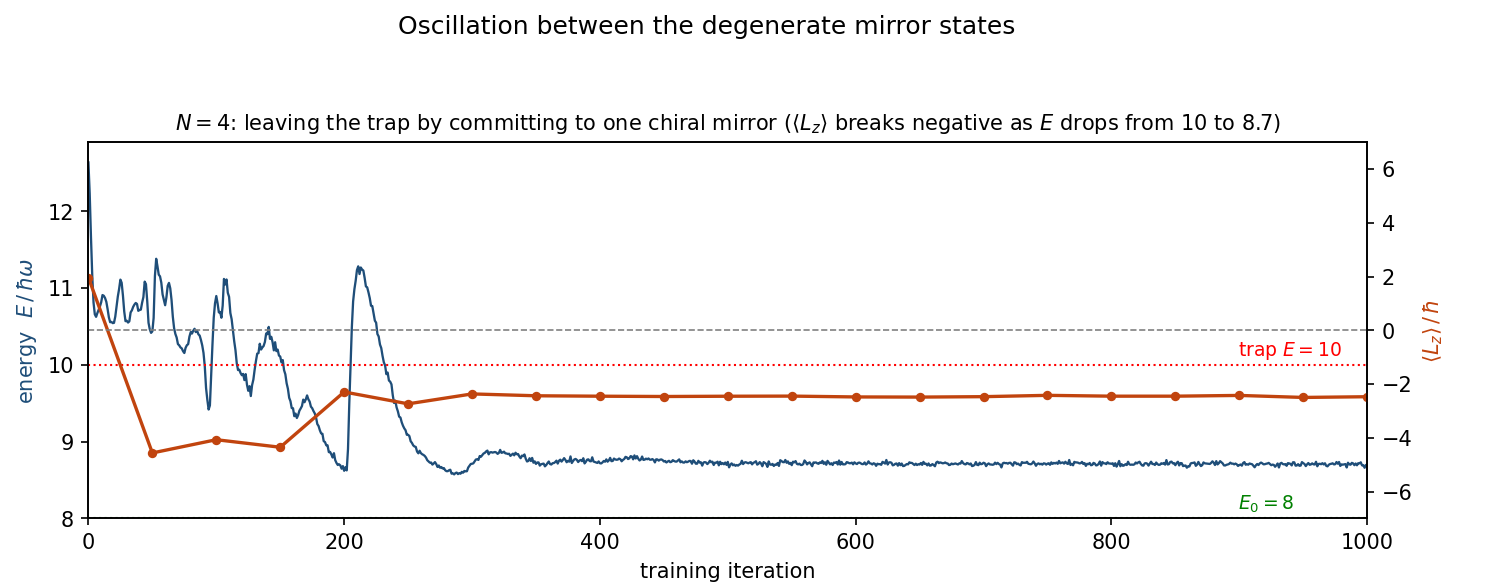
\includegraphics[width=1\linewidth]{n4_mirror_flip.png}
    \caption{Symmetry breaking between the degenerate mirror states for $N=4$. Top: energy (blue, left axis) and angular momentum $\langle L_z \rangle$ (orange, right axis) against training iteration for a $256$-unit run.}
    \label{fig:n4_mirror_flip}
\end{figure}

\newpage

\subsubsection{The trap is not an artefact of rotational symmetry}
\label{sec:aniso}

Everything so far has been shown in the isotropic harmonic trap, which is rotationally symmetric, and one might reasonably worry that the whole phenomenon is a peculiarity of that symmetry. The holomorphic and antiholomorphic states are degenerate precisely because the trap does not distinguish the two senses of rotation, and perhaps it is only this accidental degeneracy that the network is exploiting. To rule this out we repeat the experiment on the anisotropic trap of Section~\ref{impl:sys}, $V = \tfrac{1}{2}\sum_i (x_i^2 + \omega_y^2 y_i^2)$ with $\omega_y = 1.5$, which breaks rotational symmetry outright: now $[\hat H, \hat L_z] \neq 0$, angular momentum is no longer a good quantum number, and the mirror degeneracy is gone entirely. The trap stays exactly solvable, since the two Cartesian directions still separate, and the choice $\omega_y = 1.5$ keeps the Fermi level non-degenerate, giving an exact ground-state energy $E_0 = 6.25$ for $N=3$.

The trap survives the loss of symmetry, and it survives it in a sharper form than one might have guessed. From a random start the network converges to $E = 6.75$, an eigenstate two levels above the ground state, and an overlap measurement identifies it without ambiguity: the trained state has fidelity $\mathcal{F} = 0.999$ against $\det\{1, x, x^2\}$ times the anisotropic Gaussian envelope, with essentially no weight on the true ground state $\det\{1, x, y\}$. This is once again a state whose antisymmetric part is a pure product of pairwise coordinate differences, only now assembled from the real coordinate $x$ rather than the complex $z$: it is the one-dimensional Vandermonde $\prod_{i<j}(x_i - x_j)$ embedded in the plane. It is exactly the sortable sign structure of Section~\ref{sec:lazy_trap}, and the network reaches it for exactly the same reason as before, namely that it is the antisymmetry the fixed factor $\eta$ can supply most cheaply. What changes between the two traps is only which pairwise-product eigenstate happens to be lowest; what does not change is the ansatz's preference for pairwise-product sign structures over the genuinely two-dimensional, signed-area sign structure that the true ground state requires. The pathology is therefore a property of the parity-graded construction and its optimisation, not of the rotational symmetry of any one trap.

Because rotational symmetry is broken, the projection remedy of the next section cannot be applied to this trap directly: there is no conserved $L_z$ left to project onto. 





\subsection{Comparison with a learned determinant}
\label{sec:slater_comparison}

The trap and the wall are both properties of how FermiSets builds antisymmetry, so the natural way to put them in perspective is to run the same pipeline with antisymmetry built the standard way, from a learned determinant. The SlaterNN baseline of Section~\ref{sec:slaternn} shares everything with FermiSets except the antisymmetrisation mechanism: the same continuous-space sampler, the same SR driver, the same Gaussian envelope and the same training budget, differing only in that its nodal surface is a determinant of learned orbitals rather than a fixed Vandermonde factor dressed by a symmetric network. Table~\ref{tab:slater_vs_fermisets} places the two side by side on every system we have used.

\begin{table}[H]
    \centering
    \begin{tabular}{l r r r}
        \hline
        system & FermiSets & SlaterNN & reference \\
        \hline
        $N=3$ QHO  & $5.015$ ($0.3\%$)          & $4.99997$ ($0.0006\%$) & $5.0$ (exact) \\
        $N=6$ QHO  & $\approx 16$--$17$ (stall)  & $13.9994$ ($0.004\%$)  & $14.0$ (exact) \\
        $N=6$ dot  & $20.19$ ($6.2\%$)          & $19.165$ ($0.85\%$)    & $19.004$ (ED) \\
        \hline
    \end{tabular}
    \caption{FermiSets, with $L_z$ projection where applicable, against the SlaterNN baseline, both from scratch and at a single seed. The FermiSets $N=3$ entry is the projected run of Section~\ref{sec:lz_projection}; its $N=6$ entries are the best energy reached within budget, none of which converge. SlaterNN reaches the ground state to within a fraction of a percent on every system.}
    \label{tab:slater_vs_fermisets}
\end{table}



\newpage

\section{Conclusions $\&$ Outlook}
\label{sec:conclusions_outlook}
\subsection*{Conclusions}

The two ansätze we have compared differ in one fundamental respect, namely how antisymmetry, and with it the nodal surface of the wavefunction, is realised, and this single difference accounts for almost everything we observed.

In SlaterNN the antisymmetry is enforced through a determinant $\det[\phi_i(r_j)]$ whose single-particle orbitals $\phi_i$ are themselves learned functions. The entire nodal surface, the set where $\psi = 0$ that fixes the sign structure of the wavefunction, is therefore a free function of the network parameters. The optimiser is tied to no particular sign structure in advance and can continuously reshape the nodes toward whatever the true ground state requires, which is why SlaterNN reaches the ground state on every system we tested and never falls into a chiral trap.

As a contrast, FermiSets has a rigid nodal set, unlearnable directly by the network. Across every system studied, the FermiSets ansatz fails from a random
start in a single, reproducible way: it converges to the state whose
antisymmetry its fixed factor $\eta$ can supply most cheaply. At $N=3$
and $N=4$ in the isotropic trap this is the holomorphic Vandermonde
state at $E = N(N+1)/2$, identified against the analytic reference at
$\mathcal{F} \approx 0.85$ and $0.95$; in the anisotropic trap, where
no rotational degeneracy exists, it is the real one dimensional
Vandermonde $\det\{1,x,x^2\}$ at $\mathcal{F} = 0.999$. The trap is
therefore not an artefact of rotational symmetry, nor of any one
Hamiltonian, but of the pairwise product sign structure the
construction imposes. It is also not a tuning artefact: across $76$
from-scratch runs at widths from $16$ to $512$ units, capacity bends
the trap without breaking it, the best stable energy at $N=4$
remaining $E \approx 8.36$ against $E_0 = 8$, while the larger widths
destabilise the stochastic-reconfiguration update rather than
improving on it.

Projecting the ansatz onto the $L_z = 0$  removes the trap from the space the optimiser can explore, at a cost of $O(K N^2)$ against the $O(N^3)$ of a Slater
determinant, which unfortunately does not scale for any system with $N>3$. The reason it does not is a second and independent problem. At $N=6$ the projected network stalls at $E \approx 16$ to $17$ for every projection order tried, including orders that leave the trap inside the allowed sector and orders that
remove it. Since removing the trap does not change where the network
lands, the plateau is not the trap but it is built from
excited states below the trap, against which symmetry projection is powerless by construction. Supervised pretraining locates the obstruction in
representability rather than in optimisation: the overlap with the
exact ground state falls monotonically with the number of occupied
shell-$2$ orbitals, from $0.91$ at $N=3$ through $0.80$ and $0.11$ to
numerically zero at $N=6$ and beyond, and neither budget, width, nor
the choice of degenerate member moves it. Those are precisely the
orbitals whose nodal structure is not holomorphic, which is what the
fixed $\eta$ cannot supply.

All in all, the trap is a property of the optimisation landscape induced by a holomorphic
signature encoder, and symmetry projection removes it. The wall is a
property of the encoder itself, and no amount of symmetry, capacity or
budget removes it. That both trace to the same fixed factor is
confirmed by the learned-determinant baseline, which shares every
component of the pipeline except the antisymmetrisation mechanism and
reaches the ground state to better than one percent on every system in
the study.

\newpage
\subsection*{Outlook}


The wall we have measured may well be specific to the architecture we
studied rather than to the whole family it belongs to. Our ansatz uses
a single fixed antisymmetric factor, and it is exactly that choice
that makes the node of $\eta$ a floor the symmetric network cannot
lift. More recent constructions \cite{fu_fermi_2026} keep exact
antisymmetry and the $O(N^2)$ cost while relaxing this restriction,
either by combining several antisymmetric factors or by learning them
instead of fixing them in advance. Whether that is enough to reach the
ground states we could not represent is an open question, and a cheap
one: the supervised assay of Section~\ref{sec:pretraining} would
answer it in a single run per system.

\newpage
\part{Appendix}
\appendix

\section{Optimizer and Hyperparameter Ablations}
\label{app:ablations}

These are tuning and engineering choices made along the way, not results the thesis's claims depend on; kept here for reproducibility.

\subsection{Test of Optimizers}

Since we had significant troubles with instabilities within the SR driver, we also tested the very standard, general Machine Learning approach of using the Adam Optimizer without Stochastic Reconfiguration. Since we don't have to compute the S matrix, that allowed us to fit a much bigger model on the same GPU.
Instead of having $[16,32,64]$ hidden units we used $[16,32,1024]$, and additionally added one extra layer with weight dimension $[\texttt{hidden\_size} \times \texttt{hidden\_size}]$.

We report that adding the extra layer (even when reduced in size) increased training time massively (30 times more per iteration), which we attribute to the way the code is parallelized in our setup.

The setup with Adam and no SR did not have numerical instability troubles and found the Laughlin state with low errors of around 0.001 percent, but couldn't converge to the actual ground state.

\paragraph{Solver for SR Optimizer}

However, the inverse is often ill-defined. One reason is that Monte Carlo estimates of matrix elements are noisy. Noise accumulates to render the matrix singular by making small eigenvalues vanish. Therefore, quickly and efficiently obtaining many uncorrelated samples is crucial. \cite{medvidovic_variational_2023}

\label{sec:solver}
\subsection{Hyperparameter Optimization}
\paragraph{Effect of hidden layer size}

The effect of hidden-layer width on the $N=4$ QHO benchmark is presented as a result in the main text (Figure~\ref{fig:n4_convergence} and Table~\ref{tab:width_scaling}, Section~\ref{sec:brute_force}), since it bears directly on the trap rather than being a mere tuning choice.

The best \texttt{diag\_shift} is 0.001, with the soft-SVD optimiser.
\paragraph{Regularisation of antisymmetric part}

In our formulation of the antisymmetric function, Equation~\ref{eq:eta}, which is regularised by the parameter $a$, we made a quick sweep to assess its effect:

TODO

\section{Architectural variants against the $N=6$ wall}
\label{app:variants}

The $N=6$ wall of Section~\ref{sec:n6_wall} is a limit of the fixed signature encoder, and the obvious response is to give that encoder more freedom. We tried two such variants and record them here rather than in the main text, since neither changes the conclusion: the wall stands in both cases. Both were assessed with the supervised fit of Equation~\ref{eq:supervised_loss}, which isolates representability from the optimisation dynamics of a full VMC run, and both were checked against an $N=3$ control on the same machinery, so that a null result at $N=6$ could not be blamed on a broken metric.

The first variant adds a pairwise feature stream to the symmetric part: a Deep Sets network over the $N(N-1)/2$ unordered pairs, with exchange-even features of each pair distance, among them $\log(r^2 + \varepsilon)$, which gives the symmetric network linear access to the singular denominator that a signed-area sign structure needs, pooled and concatenated into $\xi$ before the $\Psi$ head. Enabling it (\texttt{pair\_hidden}) lowers the amplitude loss at both $N=3$ and $N=6$, confirming that it does add representational power to the symmetric factor, but it leaves the phase loss essentially unchanged, near $1$ at $N=6$ and around $0.3$ at $N=3$ (Table~\ref{tab:variants}). This is what one expects on reflection: the pair features are real and exchange-even, so they enrich the modulus of the wavefunction but never touch the sign structure, which lives entirely in $\eta$.

The second variant makes the signature encoder itself trainable through a backflow. The raw coordinates entering $\eta$ are replaced by $\tilde z_i = z_i + \Delta_i$, where $\Delta_i$ is a permutation-equivariant Deep Sets map of all particle positions, so that $\eta(\tilde z)$ stays exactly antisymmetric while its nodal surface becomes a learned, and no longer holomorphic, function. This is the more powerful of the two, since it attacks the sign structure directly, and at $N=3$ it produces the best supervised fit of any variant we tried, driving the phase loss down to $0.02$, essentially an exact match. At $N=6$, however, the phase loss stays pinned near $1$, exactly as for the plain and pair-augmented ansätze. The failure is not for want of trying on the network's part: the trained deformation is large, of the same order as the coordinates themselves, and it shifts the phase of the signature substantially, yet none of it reaches the target sign structure. The $N=6$ ground state remains out of reach even when the encoder's coordinates are free to move.

\begin{table}[H]
    \centering
    \begin{tabular}{l r r}
        \hline
        variant ($N=6$, hidden $64$) & amplitude & phase \\
        \hline
        plain              & $1.04$ & $0.99$ \\
        pair stream        & $0.76$ & $1.01$ \\
        signature backflow & $0.88$ & $0.99$ \\
        \hline
        \multicolumn{3}{l}{\emph{$N=3$ control, phase loss:} plain $0.20$, pair $0.32$, backflow $\mathbf{0.02}$} \\
        \hline
    \end{tabular}
    \caption{Supervised fit (Equation~\ref{eq:supervised_loss}) of the plain ansatz and its two variants to the exact ground state. At $N=6$ every variant leaves the phase loss pinned near $1$, so none is able to represent the ground-state sign structure; the $N=3$ control shows that all three can fit that smaller system, backflow best of all, ruling out a metric artefact.}
    \label{tab:variants}
\end{table}

The lesson these two variants share is the one drawn in the Outlook. A pairwise product of coordinate differences, whether its coordinates are fixed or deformed by a backflow, carries a sign structure of a fixed pairwise character, and the two-dimensional, signed-area nodes of the true $N=6$ ground state appear to lie outside what any such product can represent. Lifting the wall, if it can be lifted within the $O(N^2)$ budget, seems to require changing the product structure of the signature and not merely the coordinates fed into it.

\bibliographystyle{ieeetr}
\bibliography{zotero_references}
%\printbibliography
\end{document}
